\documentclass{article}

\usepackage{ijcai15}

\usepackage{times}
\usepackage{comment}

\usepackage[pdftex]{graphicx}
\usepackage{comment}

\usepackage{algorithm}
\usepackage[noend]{algpseudocode}

\usepackage{amsfonts}
\usepackage{amsmath}
\usepackage{bm}
\usepackage{float}

\usepackage{amsthm}
\newtheorem{thm}{Theorem}
\newtheorem{lem}{Lemma}
\newtheorem{asmp}{Assumption}
\newtheorem{defn}{Definition}
\newtheorem{clm}{Claim}

\usepackage{caption}
\usepackage{subcaption}

\title{ MORRF$^*$: Sampling-Based Multi-Objective Motion Planning }

\author{Author Names Omitted for Anonymous Review.}

\begin{document}

\maketitle

\begin{abstract}
Many robotic tasks require solutions that maximize multiple performance objectives.  
For example, in path-planning, these objectives often include finding short paths that avoid risk and maximize the information obtained by the robot.  
Although there exist many algorithms for multi-objective optimization, few of these algorithms apply directly to robotic path-planning and fewer still are capable of finding the set of Pareto optimal solutions.  
We present the MORRF$^{*}$ (Multi-Objective Rapidly exploring Random Forest$^{*}$) algorithm, which is blends concepts from two different types of algorithms from the literature: Rapidly exploring random tree (RRT$^{*}$) for efficient path finding~\cite{Karaman.Frazzoli:RSS10} and a decomposition-based approach to multi-objective optimization~\cite{4358754}.  
The random forest uses two types of tree structures: a set of {\em reference trees} and a set of {\em subproblem trees}.  
Each reference tree explores a single objective, and the estimates from the set of reference trees are used to estimate what is called the {\em Utopia reference vector}. This vector is required by the multi-objective optimization part of the algorithm.  
Each subproblem tree explores the space, seeking to find an optimal solution to the subproblem created by blending different objectives.  
We present a theoretical analysis that demonstrates that the algorithm asymptotically produces the set of Pareto optimal solutions, and use simulations to demonstrate the effectiveness and efficiency of MORFF$^{*}$ in approximating the Pareto set.
\end{abstract}

\begin{comment}
[Brief abstract submission] - February 8, 2015 (11:59 UTC-12)
[Final paper submission] - February 12, 2015 (11:59 UTC- 12)

Submitted technical papers must be no longer than seven pages in total: 
six pages for the main text of the paper (including all figures but excluding references), 
and one additional page for references. 
Note that the references page should only include references. 
\end{comment}

\section{Introduction}
\label{sec:intro}

Many tasks assigned to robots are complex, can be performed in several different ways, and must maximize several different performance objectives.  
For example, a robot in a search task may be expected to maximize the area that covers while minimizing energy consumption and avoiding risk (see, for example~\cite{yi2014supporting,mei2005deployment}). 
As another example, a robot manipulator may need to satisfy performance criteria related to movement, joint velocities, joint accelerations, etc.~\cite{Pires2004}.

%In many real applications of the robots, the complexity of tasks inherently implies more than single objective to be reached.
%A robot in a search task is usually expected to maximize the search coverage with a consideration of the energy efficiency so that the execution time could also be expanded~\cite{yi2014supporting}. 
%If there exists risk in the working environment, the robot should also try to avoid dangerous regions.
%In robot arm manipulation planning, there usually exist several criteria to be considered as well~\cite{Pires2004}, for example, movement, joint velocities, joint accelerations and etc. 

A common method for finding a solution to a multi-objective optimization problem is to optimize a single objective created by a weighted sum of the multiple objectives.  
In path-planning the properties of the path produced by this method depends strongly on how each objective is weighted. This means that either the programmer, designer, or a human teammate must decide how to assign the weights so that the qualitative behavior matches what is intended.  
In addition to the burden this places on the human operator, optimizing a weighted sum does not work when the multiple objectives are very difficult to compare or are expressed in incommensurate units.

In response to these challenges, it is useful of find {\em the set of payoff dominant solutions} to the multi-objective path-planning problem, meaning the set of solutions for which there is no other solution that produces better payoffs for every objective.   
This paper uses the economics term {\em Pareto optimal} to denote a payoff dominant solution.  Although not demonstrated in this paper, we propose that if an algorithm could produce the set of Pareto optimal solutions then a human could interactively explore this set to find one or more solutions that matches his or her expectations. 
The objective of this paper is to create an algorithm that efficiently finds the Pareto set in a multi-objective path-planning problem.

Most popular methods in multi-objective optimization do not naturally apply to path-planning problems~\cite{4358754,6600851}.
%{\sc Give a reference to a good review or a reference to a handful of representative multi-objective methods}
The main reason for this is that path-planning often represents the problem to be solved as a semi-structured tree with an exponential number of possible trajectories through the tree, and the number of evaluations of the objective function required by existing algorithms do not scale well when there are an exponential number of solutions. 
One approach to addressing this issue is to change the representation for a path by, for example, coding a path as a sequence of fixed-length line segments represented by direction~\cite{Ahmed2013,howlett2006learning} or waypoints~\cite{5160222,Pires2004}.  
This produces an encoding that can be ``fed into" an appropriate evolutionary algorithm to search for the Pareto set. 
Unfortunately, these approaches do not scale well for large problems because the number of segments required to represent the paths grows too quickly, and estimating the required number of segments {\em a priori} is very challenging.  
Another approach to solving the multi-objective path-planning problem is to represent the path as a point in a very high-dimensional vector space. In this approach a path is represented as a point in a $ n * d $ dimensional space formed by $ n $ $ d $-dimensional way-points. If the number of way-points can be held constant, we can use standard approaches to explore the space. However the search can be more difficult if we allow the number of way-points, and therefor the dimensionality of the optimization problem, to vary.
Indeed, we will use this as to guide our solution, but the algorithm we present works when the obstacles in the path-planning space introduce discontinuities in these high-dimensional spaces, which limits the applicability of heuristic-based search approaches~\cite{5160222,4358754}.

The RRT (Rapidly exploring Random Tree) algorithm is popular for finding feasible solutions from a start position to a goal position in continuous or very large search spaces; it also works well when environments have complex obstacles. 
The reason that RRT is popular is that the tree structure tends to be find solutions very efficiently.
The RRT$^{*}$ algorithm was a recently introduced modification to RRT that is guaranteed to find an optimal path given enough sampling time~\cite{Karaman:2011:SAO:2000201.2000209,Karaman.Frazzoli:RSS10}.

The remainder of the paper presents the MORRF$^{*}$ (Multi-Objective Rapidly exploring Random Forest*) algorithm, which we used to find a set of Pareto optimal paths from a start position to a goal position.  
MORRF$^{*}$ blends concepts from RRT$^{*}$ a decomposition-based approach to multi-objective optimization~\cite{4358754}.  
The random forest uses two types of tree structures: a set of {\em reference trees} and a set of {\em sub-problem trees}.  
Each reference tree explores a single objective, and the estimates from the set of reference trees are used to estimate what is called the {\em Utopia reference vector} required by the adapted multi-objective optimization algorithm.  
Each sub-problem tree explores the space, seeking to find an optimal solution to the sub-problem created by blending different objectives. 

The paper is structured as follows.  
Section~\ref{sec:related_works} reviews relevant work in multi-objective optimization and RRT-like path-planning. 
Section~\ref{sec:morrt} presents the MORRF$^{*}$ algorithm,  
Section~\ref{sec:theoretic_analysis} proves that the algorithm produces the Pareto frontier given enough sampling time, 
and Section~\ref{sec:simulation} uses simulations to illustrate the algorithm's performance.

\section{Related Work}
\label{sec:related_works}

An algorithm that discovers the set of Pareto optimal solutions must discover those solutions for which no other solution is better with respect to every objective.  A naive algorithm would do this by comparing every solution to every other solution, which works for problems with a small, discrete set of solutions, but does not work for continuous spaces or problems with exponential numbers of potential solutions.  
Marler and Arora observed that ``no single approach is superior [for all problems].  
Rather, the selection of a specific method depends on the type of information given in the problem"~\cite{marler2004survey}.  
We note that (single objective) path-planning in a continuous state space is often efficient using RRT* or other discretization-based approaches. This suggests that we use a discretization-based approach, ruling out, for example, variational approaches to solving the problem.    

Prior work has modeled the search space as a graph and applied a multi-objective A* search to find the solution~\cite{Mandow:2005:NAM:1642293.1642328}. 
The limitation of this approach is that it requires an {\em a priori} discretization rather than a discretization that is guided by the objectives as is done in RRT$^{*}$; a coarse discretization throws away potentially valuable information and a fine discretization increases complexity and adds redundancy in the resulting graph structures.
Obstacles can make it more difficult to determining which cells in the discretized space are connected to which others, especially when searching a space of more than 2 dimensions such as in planning the trajectory for a robotic manipulator.
Another approach that users an {\em a priori} discretization (and suffers from these limitations) is to encode a path as a sequence of directions from one cell to next cell and then using the NSGA-II algorithm to find a set of Pareto optimal solutions \cite{Ahmed2013}.  
Constrained splines have been introduced to interpolate a sequence of way points into a trajectory that avoids obstacles~\cite{6181426}, but the effect of the interpolation on the quality of the solution has not been evaluated.
In addition to the genetic approach used in NSGA-II, evolutionary algorithms based on the decomposition method have also been proposed ~\cite{6600851}.

% Evolutionary algorithms can be used to fine the Pareto set, but these approaches tend to be inefficient when applied to spaces with high dimensions~\cite{marler2004survey}.  For such spaces, small deviations in possible solutions may need to be considered in order to find an optimal solution, but this means exploring many possible solutions for problems with non-linearities or multiple local maxima.   A path in a fixed-length search tree of depth $d$ can be considered as a point in $\Re^d$, so tree-based approaches followed by an evolutionary "fine-tuning" stage risk running into the problems just listed with evolutionary approaches. 

In contrast to searching through and comparing solutions in order to find the Pareto optimal set, decomposition-based methods provide an attractive alternative.  
In this paper we uses a decomposition-based method similar to MOE-D~\cite{4358754}.  
MOEA-D is an algorithm that decomposes a multi-objective optimization problem into a set of subproblems.  
Each subproblem uses a weighed combination of the objectives to find specific points in the Pareto set or to guide the search for such points.  
Because we  will use this subproblem idea in our algorithm, it is useful to introduce some notation.
Let $ \bm{\lambda} = [ \lambda_{1} , \cdots , \lambda_{K}  ]^{T} $ be a weighting vector such that $ \sum_{k=1}^{K} \lambda_{k} = 1 $.  Let $\{c_{1}(\cdot), c_{2}(\cdot), \ldots c_{K}(\cdot)\}$ denote the K-element set of objective functions, let $F(x) = [c_{1}(x), c_{2}(x), \ldots, c_{K}(x)]^T$, and let $x$ denote a potential solution.  Finally, let $ \bm{z}^{\rm utop} = [z^{*}_{1}, \cdots , z^{*}_{K}]^{T} $ denote the so-called ``Utopia" reference vector, described in more detail in the next section. 
Three types of decomposition methods have been used in prior work~\cite{4358754}; however we will use only the two methods described below, leaving the third (the boundary intersection method) to future work.
\begin{eqnarray}
 \arg\max_x \sum_{k=1}^{K} \lambda_{k} c_{k} (x) & {\rm weighted \ sum} \label{eq:weighted}\\
 \arg\min_x\max_{1 \leq k \leq K}  \{ \lambda_{k} \mid c_{k}(x) - \bm{z}^{\rm utop}_{k}  | \} & {\rm Tchebycheff} \label{eq:Tchebycheff}%\\
 %\arg\min_x \{ d \mid \bm{z}^{\rm utop} - F(x) = d \bm{\lambda} \} & {\rm boundary \ intersect\ } \label{eq:boundary}
\end{eqnarray}
%\begin{itemize}
%\item \emph{Weighted sum}:
%Maximize $ g^{ws} (x \mid \bm{\lambda}) = \sum_{k=1}^{K} \lambda_{k} c_{k} (x) $;
%$\arg\max_x \sum_{k=1}^{K} \lambda_{k} c_{k} (x) $;
%\item \emph{Tchebycheff}:
%Minimize $ g^{te} (x \mid \lambda , \bm{z}^{\rm utop}) = \max_{1 \leq k \leq K}  \{ \lambda_{k} | c_{k}(x) - z^{*}_{k}  | \} $;
%$\arg\min_x\max_{1 \leq k \leq K}  \{ \lambda_{k} | c_{k}(x) - \bm{z}^{\rm utop}_{k}  | \} $;
%\item \emph{Boundary intersection}:
%Minimize $ g^{bi} (x \mid \lambda , \bm{z}^{\rm utop} ) = d $, subject to $ \bm{z}^{\rm utop} - F(x) = d \lambda $.
%$\arg\min\{d \mid \bm{z}^{\rm utop} - F(x) = d \lambda $\}.
%\end{itemize}
The solutions generated by each method are a subset of the Pareto optimal set.

Sampling-based path planning works effectively in continuous space. 
The RRT (Rapidly exploring Random Tree) has been one of the most popular tools, which  efficiently explores the space by randomly sampling the search space; this algorithm tends to work well in the presence of complex obstacles.
Unfortunately, RRT has been shown to fail in certian conditions~\cite{Karaman.Frazzoli:RSS10}. 
In response, the RRT$^{*}$ algorithm was proposed, which uses a \emph{Rewire} process to gradually update the tree structure when new samples of the space indicate that this is needed. Thus RRT$^{*}$ is asymptotically
optimal~\cite{Karaman.Frazzoli:RSS10}~\cite{Karaman:2011:SAO:2000201.2000209}. 

\section{Multi-Objective Rapidly exploring Random Forest$^{*}$}
\label{sec:morrt}

Consider a multi-objective path planning problem defined on a bounded, connected open set $X\subset\mathbb{R}^d$ of possible solutions, and $K$ different objectives $\{c_{1}(\cdot), c_{2}(\cdot), ... c_{K}(\cdot)\}$. 
Without loss of generality, we assume that each $c_{k}(\cdot)$ is a cost function so that our objective is to minimize these functions.  
Since the Pareto optimal set is not enumerable, our {\em goal is to find a representative, finite ($M$-element) subset of the Pareto optimal set}.  
By ``representative" we mean that we want a diverse set of solutions that span the Pareto set rather than, for example, several points clustered in a single region of the Pareto set.  

\begin{defn}{ \textbf{Multi-Objective Path Planning} }
Consider a bounded, connected open set $ X \subset \mathbb{R}^{d} $, an obstacle space $ X_{obs} $, an initial state $ x_{init} $, and a goal region $ X_{goal} $. 
Consider the set of $K$ objectives determined by a vector function $ \bm{F}(\cdot) = [ c_{1} (\cdot), \ldots , c_{K}(\cdot) ]^{T}$ defined by $\bm{F}: \mathbb X \rightarrow \mathbb{R}^{K} $. 
Denote the obstacle-free space by $ X_{\it free} = X \setminus X_{obs} $. Note that $\bm{F}$ is defined for all points in $X$ both those in free space and obstacle space.

Define a {\em path} in $X$ as a continuous curve parameterized by $s$, denoted by $\sigma : [0,s] \rightarrow X$. 
Define the cost of the path as the vector-valued function $ \bm{F}(\sigma) = \int_{\sigma} \bm{F}(x)ds $.  
The goal is to find $ M $ Pareto optimal paths $ \sigma^{*} \in \Sigma^{*}$ such that
\begin{itemize}
	\item $\forall \tau\in[0,s], \sigma^*(\tau) \in X_{\it free}$;
	\item $ \sigma^{*} (0) = x_{init} $ and $ \sigma^{*} (s) = X_{goal}  $;
	\item There does not exist $ \sigma $ that,
	\begin{itemize}
		\item $ \forall k \in K, c_{k} (\sigma) \leq c_{k} (\sigma^{*}) $;
		\item $ \exists k' \in K, c_{k'} (\sigma) < c_{k'} (\sigma^{*}) $.
	\end{itemize}
\end{itemize}
\end{defn}
\noindent Without loss of generality, we could set $s=1$ for all paths, but we retain the $s$-parameter because it is a convenient way of signalling that two paths may be different lengths.  Note that this last condition enforces a very strict form of payoff dominance; extensions to the algorithm can be made for weaker forms of payoff dominance.

Adopting the idea from the MOEA-D algorithm~\cite{4358754}, the $M$ elements in the solution set $\Sigma^{*}$ will be obtained by decomposing the multi-objective problem into $ M $ subproblems.  
In this paper, we implement only the Tchebycheff approach, noting that the Boundary Intersection Approach can be used with only slight modifications to our algorithm. The Tchebycheff approach requires us to define a Utopia reference vector $ \bm{z}^{\rm utop} $ in the fitness space. 
Before describing how we find $ \bm{z}^{\rm utop} $ and how we combine the Tchebycheff approach with RRT$^{*}$, it is useful to illustrate how the reference vector is used to help find the Pareto set; Figure~\ref{fig:Tchebycheff} illustrates the process for two objectives.  
\begin{figure}
\centering
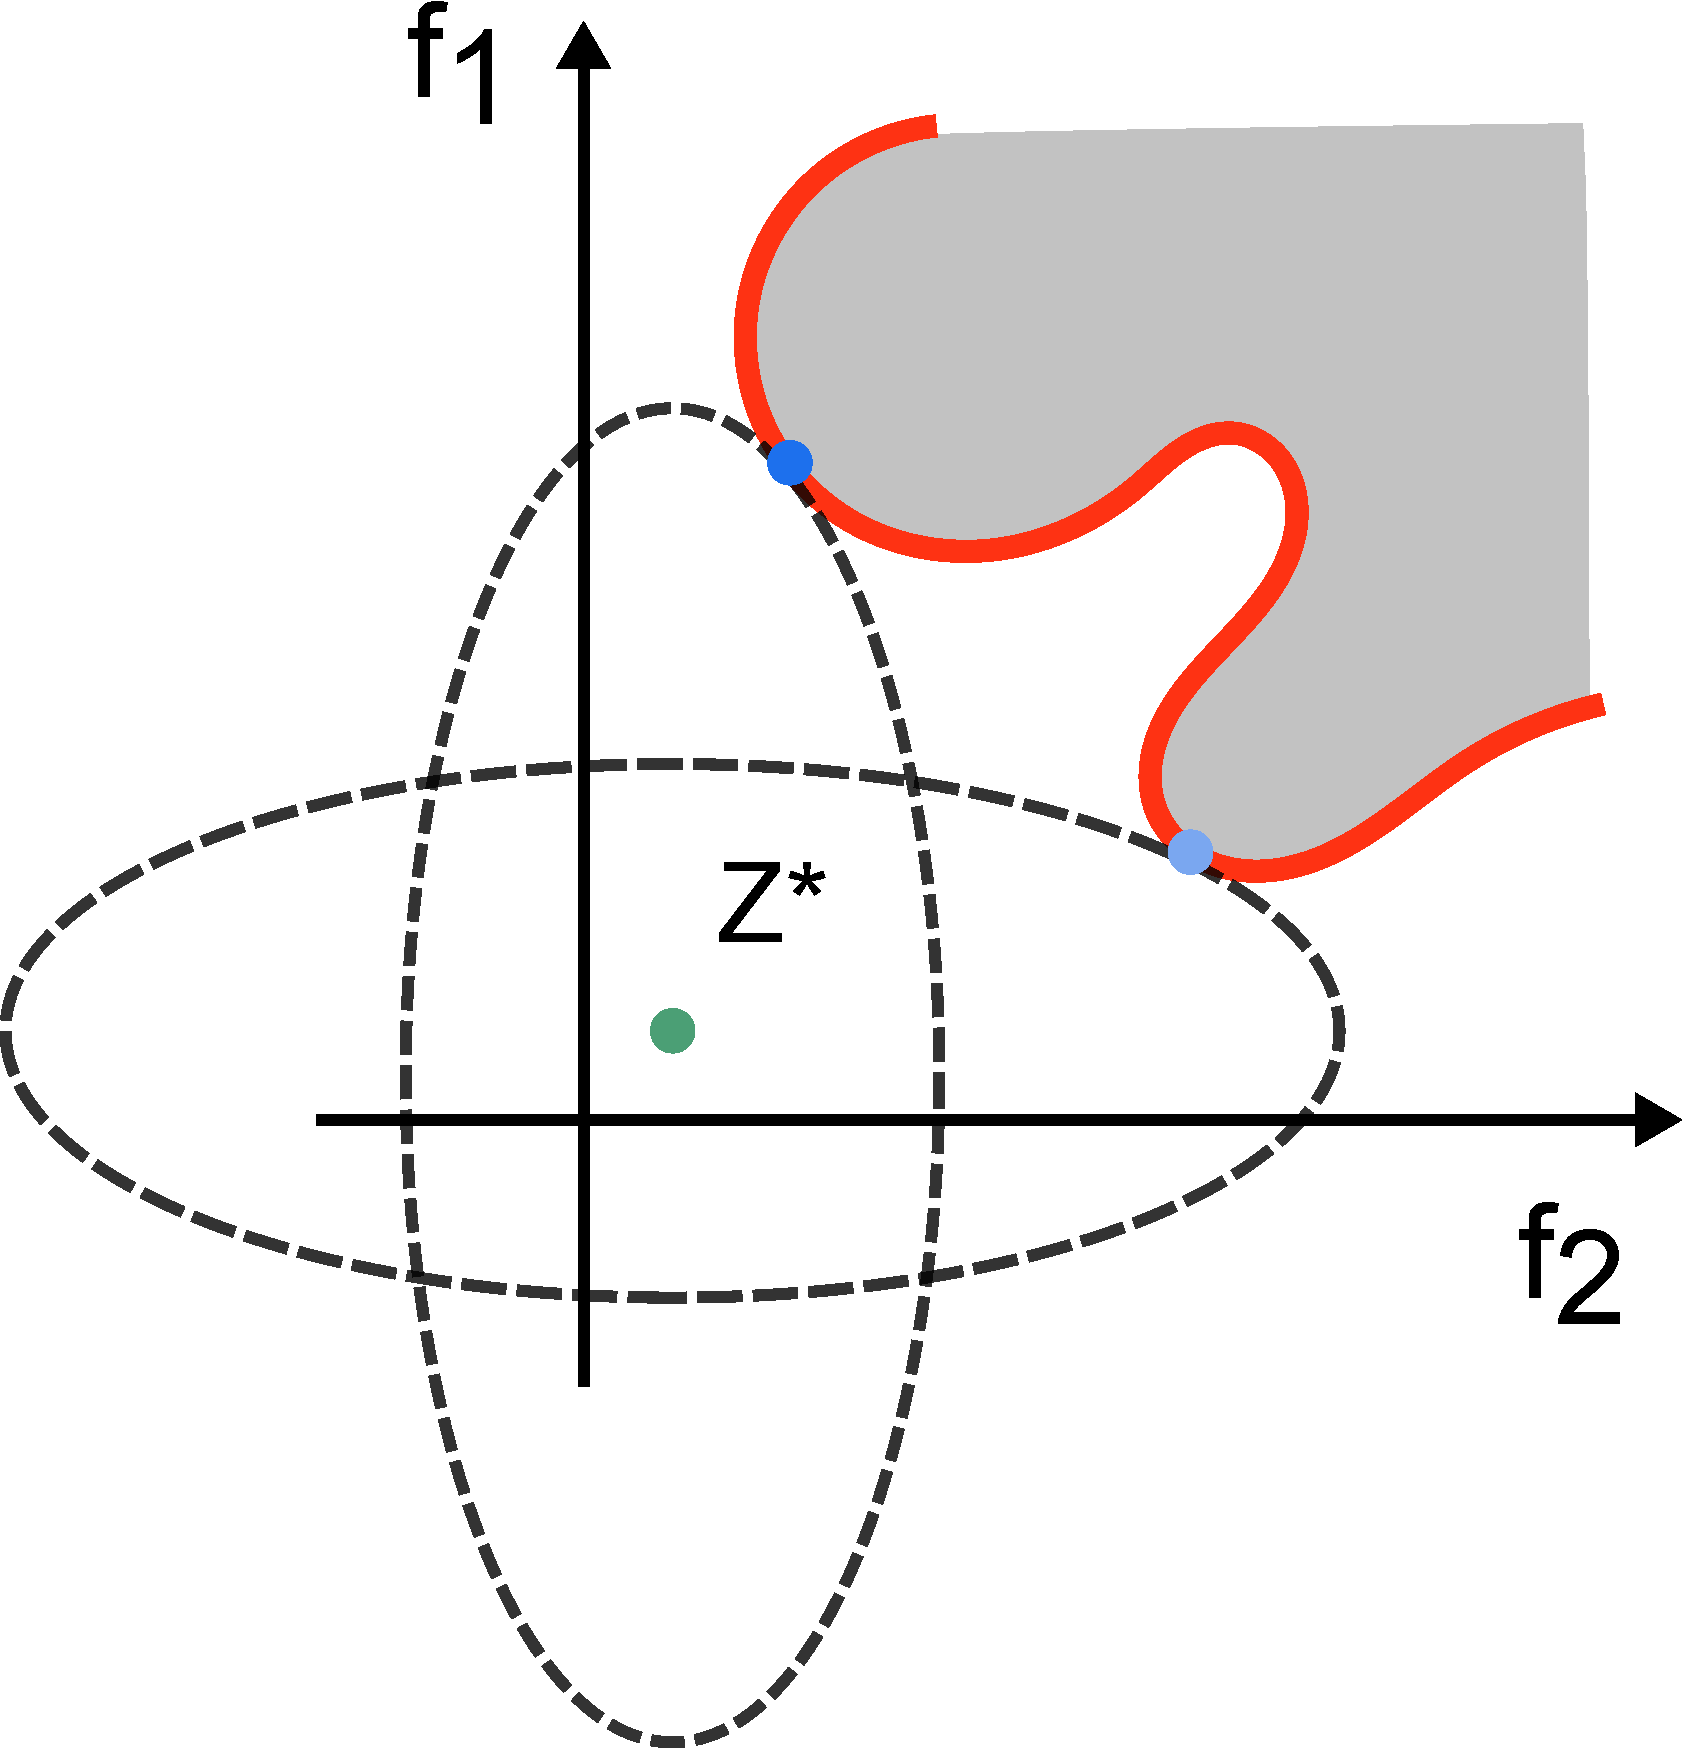
\includegraphics[width=0.4\linewidth]{fig/Tchebycheff2.png}
\caption{Tchebycheff method of finding Pareto front.}
\label{fig:Tchebycheff}
\end{figure}
Recall from the previous section that  $ \bm{\lambda} = [ \lambda_{1} , \cdots , \lambda_{K}  ]^{T} $ is a weighting vector such that $ \sum_{k=1}^{K} \lambda_{k} = 1 $ and that the Tchebycheff approach seeks to find the solution $ x^{the}\in X $ given by $ x^{te} = \arg\min_x \max_{1 \leq k \leq K}  \{ \lambda_{k} | c_{k}(x) - \bm{z}^{\rm utop}_{k}  | \} $.  
As illustrated in the Figure, the Utopia reference vector is defined as that point in reward space that would be obtained if it were possible to find a solution that produced the minimum value for all objectives, that is the $k^{\rm th}$ element of $\bm{z}^{\rm utop}$ is given by $\bm{z}^{\rm utop}_{k} = \arg \min_{x \in X} c_{k}(x)$.  
It is called the Utopia reference vector because it represents the very best that could conceivably be achieved for an ideal point in the solution space.

Given this brief overview of the Tchebycheff method, we now need to extend it to allow for RRT$^{*}$-based sampling of the search space.  
We will need one type of RRT$^{*}$ structure to explore in an attempt to find the Utopia reference vector in payoff space and another type of RRT$^{*}$ structure to find paths that minimize the Tchebycheff condition.  
Thus, there are two types of tree structures used for the optimization process.
\begin{itemize}
\item Each \emph{reference tree} explores using a single objective $ c_{k} (x), k \in K $. 
The cost of each vertex is calculated using the $ k^{\rm th} $ objective function.
\item Each \emph{subproblem tree} explores a subproblem $ g_{m} ( x \mid \lambda_{m} , \bm{z}^{\rm utop} ) , m \in M $.
The cost of each vertex is calculated using $ g_{m}(x) $ defined by the corresponding approach.
\end{itemize}
Thus $ K $ reference trees are used, one each to explore the minimum of each objective, and $ M $ subproblem trees are used, one for each weighting vector, $ \lambda_{m} $, which is described below.  
The $K$ reference trees and $M$ subproblem trees constitute the exploration forest.

We are now in a position to describe the main flow of the MORRF$^{*}$ algorithm; see Algorithm~\ref{alg:rapidly_exploring_process}.  
The first four steps initialize two trees, the reference tree with vertices and edges denoted by $V_r$ and $E_r$, respectively, and the subproblem tree with vertices and edges denoted by $V_s$ and $E_s$, respectively.  
Each reference and subproblem tree are a collection of edges and vertices, $G_r=(V_r,E_r)$ and $G_s=(V_s,E_s)$, respectively, and the collection of reference trees and subproblem trees are denoted by ${\mathbf G}_r = \{G_r: r\in \{1, \ldots, K\}\}$ and ${\mathbf G}_s = \{G_s: s \in \{q, \ldots, M\}$.  

Because this is a path-planning problem, each vertex in each tree corresponds to a physical location in configuration space.  
For the examples used later in this chapter, configuration space is a plane so the distances will all be computed using Euclidean distance. 
Note that each each tree, reference and subproblem, uses the same set of vertices, meaning they all share the same points in configuration space.  
The differences between the trees is the edge set; each reference tree and each subproblem tree has a different way of connecting the vertices.

In each iteration, $i\in\{1, \ldots, N\}$ where $N$ is the maximum number of iterations allowed by the algorithm, a new position, $x_{rand}$ is generated by randomly sampling from the configuration space.  
The set of vertices is then searched to find that vertex whose position in the plane is nearest the random point; since all trees share the same set of vertices, any tree $G\in{\mathbf G}_r \cup {\mathbf G}_s$ may be used to find the nearest point.  
The location of this vertex is labeled $x_{nearest}$.  
It is possible that the distance between the newly sampled position and the vertex nearest to this position is very large.  
A tolerance parameter, $\eta$, is used to guarantee that the distance between the vertices in the tree and the new position is within some exploration tolerance; this is accomplished in the {\sc Steer} method.  
If the distance between $x_{rand}$ and $x_{nearest}$ is less than the tolerance $\eta$, then $x_{new}=x_{nearest}$.  
Otherwise, a line segment between $x_{rand}$ and $x_{nearest}$ is constructed and the point on this line segment that is distance $\eta$ from $x_{nearest}$ becomes the new point $x_{new}$. 
This process of finding $x_{new}$ is represented in the top layer of Figure~\ref{fig:MORRTstar}, with the dashed circle around the new point indicating $\eta$.

\begin{figure}[H]
\centering
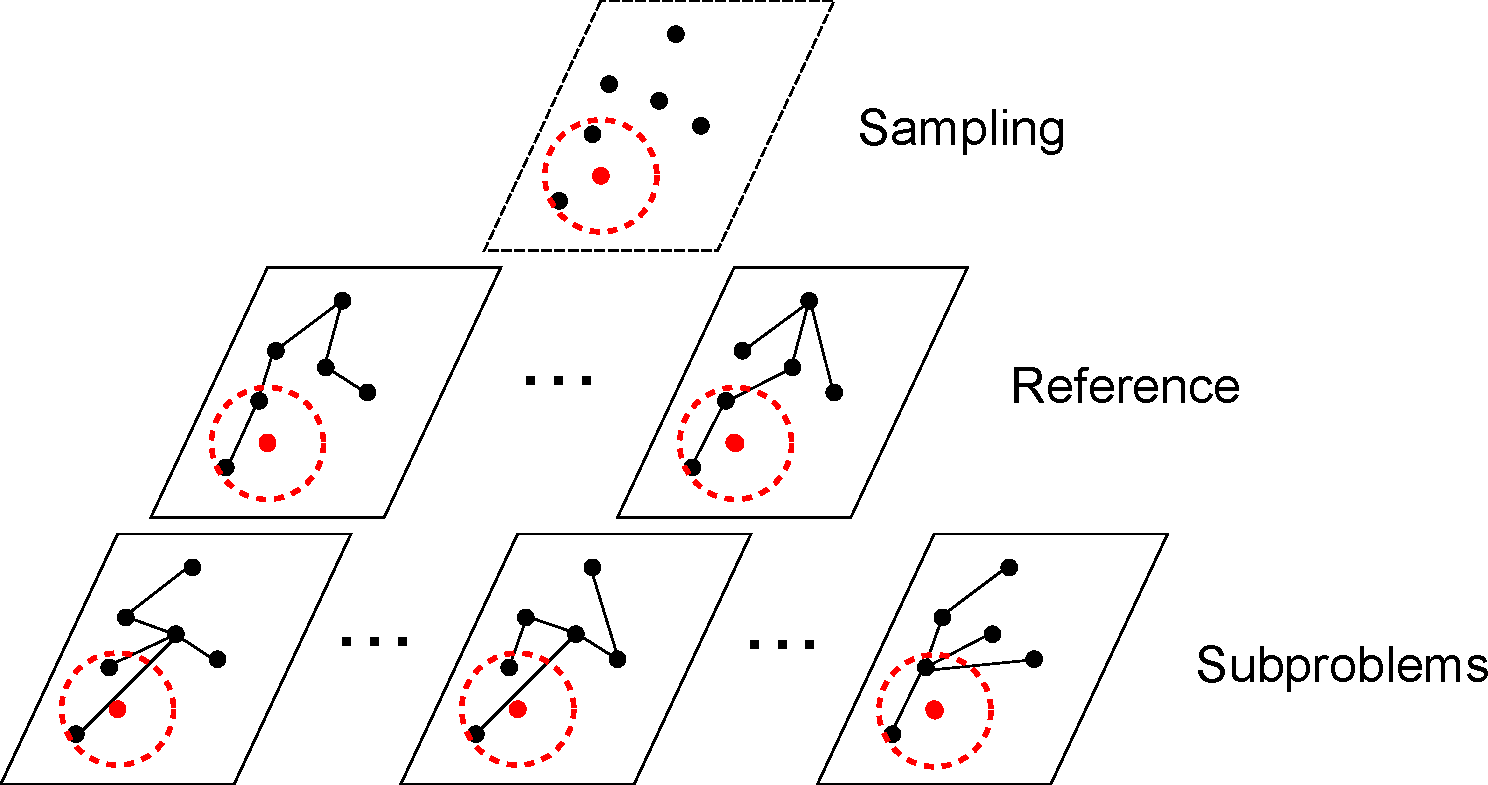
\includegraphics[width=0.7\linewidth]{./fig/MORRTstar}
\caption{Rapidly exploring process}
\label{fig:MORRTstar}
\end{figure}

Given the location of a new vertex for each tree, edges are added, potentially different edges for each reference and each subproblem tree.
We require that each new vertex be connected to some existing vertex, so a feasibility check is added using the {\sc ObstacleFree} method.
This method checks whether the line segment connecting $x_{new}$ and $x_{nearest}$ enters obstacle space.
If it does, no new vertices and no new edges are added, and another iteration of the algorithm begins. 
This check guarantees that when the algorithms are called that determine which edge to add to the reference tree or subproblem tree, there is always at least one possible edge that can be added; this is consistent with the RRT$^{*}$ algorithm.

The exploration at each iteration is given in Algorithm \ref{alg:rapidly_exploring_process}.  Like RRT$^{*}$, when the algorithm stops, each reference tree and subproblem tree returns a path, and the set of all these paths forms the solution set.

\begin{algorithm}
	\begin{algorithmic}[1]
		\For{ \textbf{each} $ V_{r} \in \mathbf{V}_{r} $ } 
		\State $ V_{r} \leftarrow \{ x_{init} \} $; $ E_{r} \leftarrow \emptyset $; $ i \leftarrow 0 $
		\EndFor
		\For{ \textbf{each} $ V_{s} \in \mathbf{V}_{s} $ } 
		\State $ V_{s} \leftarrow \{ x_{init} \} $; $ E_{s} \leftarrow \emptyset $; $ i \leftarrow 0 $
		\EndFor
		\While{ $ i < N $ }
		%\For{ \textbf{each} $ G_{r} \in \mathbf{G}_{r} $ } 
		%\State $ G_{r} \leftarrow (V_{r}, E_{r}) $
		%\EndFor
		%\For{ \textbf{each} $ G_{s} \in \mathbf{G}_{s} $ } 
		%\State $ G_{s} \leftarrow (V_{s}, E_{s}) $
		%\EndFor
		\State $ x_{rand} \leftarrow $ \Call{ Sample }{$ i $} ; $ i \leftarrow i + 1 $
		%\State $ V' \leftarrow V $; $ E' \leftarrow E $
		\State $G$ is any graph from ${\mathbf G}_r\cup {\mathbf G}_s$.
		\State $ x_{nearest} \leftarrow $ \Call{Nearest}{$ G, x_{rand} $}
		\State $ x_{new} \leftarrow $ \Call{Steer}{$ x_{nearest}, x_{rand},\eta $}
		\If{ \Call{ObstacleFree}{$ x_{nearest}, x_{new} $} }
		\For{ \textbf{each} $ G_{r} \in \mathbf{G}_{r} $ } 
		%\State $ (V_{r}, E_{r}) \leftarrow $ \Call{ Extend$_{\it Ref}$ }{$ G_{r}, x_{new}, x_{\it nearest}, r$}
		\State $ G_{r} \leftarrow $ \Call{ Extend$_{\it Ref}$ }{$ G_{r}, x_{new}, x_{\it nearest}, r$}
		\EndFor
		\For{ \textbf{each} $ G_{s} \in \mathbf{G}_{s} $ } 
		%\State $ (V_{s}, E_{s}) \leftarrow $ \Call{ Extend$_{\it Sub}$ }{$ G_{s}, x_{new}, x_{\it nearest},s $}
		\State $ G_{s} \leftarrow $ \Call{ Extend$_{\it Sub}$ }{$ G_{s}, x_{new}, x_{\it nearest},s $}
		\EndFor
		\EndIf
		\EndWhile
	\end{algorithmic}
	\caption{Multi-Objective Rapidly exploring Random Forest$^{*}$ }
	\label{alg:rapidly_exploring_process}
\end{algorithm}

We now define several functions, using appropriately modified definitions from~\cite{Karaman.Frazzoli:RSS10}.
\begin{itemize}
\item \textsc{Sample}():
Returns independent uniformly distributed samples from $ X_{\mbox{free}} $. 

\item \textsc{Nearest}():
Returns a the position of the vertex whose position is closest to point $ x $.
\textsc{Nearest}($ G = (V,E), x $) = $ \arg \min_{v \in V} \lVert x - v \rVert $.
	
\item \textsc{Steer}(): Given two points $ x $ and $ y $, returns a point $ z $ on the line segment from $x$ to $y$ that that is no greater than $eta$ from $y$. 

\textsc{Steer}( $ x,y,\eta $ ) = $ \arg \min_{ z \in \mathbb{R}^{d}, \lVert z -x \rVert \leq \eta } \lVert z - y \rVert $.

\item \textsc{ObstacleFree}(x,x): Returns True if $ [ x, x' ] \subset X_{\it free} $, which means the line segment between $ x $ and $ x' $ lies in $ X_{\it free} $.

\end{itemize}

%Because the convergence of the tree structure in RRT* means that the path from the root to any vertex is an optimal path of the defined cost.
%We use the same sampling position to extend all the trees in one iteration.
%Thus the vertices in the reference trees could be used as reference for estimating the cost in constructing the subproblem trees.

Given the general algorithm, we can now discuss how edges are added to the reference and subproblem trees.  
As illustrated in Figure~\ref{fig:MORRTstar}, second layer, edges to the reference trees are added before the edges to the subproblem trees.  
This allows us to use compute the Utopia reference vector using the path costs for each reference tree, each reference tree returning a path that approximates the minimum cost for a specific objective.  
The Utopia reference vector is then used to determine which edges should be added for each subproblem. Stated another way, the edges added to each tree are determined by the definition of the fitness (cost function) for each tree.

%Like all the sampling-based optimization, the random positions are uniformly sampled from the workspace.
%It means that all the tree have equivalent vertices constructed from same positions set sequentially.
%But they are connected by different measurements of the costs, either a single objective or a cost from subproblem definition.
%The edges of the trees can be different.

Consider the second layer in Figure \ref{fig:MORRTstar}, which shows the exploration process for the reference trees.
When a new position is obtained (red dot in Figure \ref{fig:MORRTstar}), all reference trees add a vertex that corresponds to this new location.  
Each reference tree then connects this new vertex to existing nodes by ``rewiring" a set of neighboring vertices within a specified radius (red dash circle in Figure \ref{fig:MORRTstar}).  
The process of rewiring consists of adding edges between existing vertices and the new vertex.  This is done using the {\sc Extend} method, given in Algorithm~\ref{alg:morrtstar:extend:ref}.

The idea of the algorithm is to add the new vertex, $x_{\it new}$ to the graph and then look for existing vertices in the graph that are close to the new vertex. 
Line~1 checks to see if the randomly generated position is precisely on top of the position of a vertex already in the graph.  
If so, no edges are added to the graph; this prevents self-loops, and is necessary because of finite precision numerical representations.  

Otherwise, the new vertex is added to the graph and all vertices in the graph within a particular radius are identified.  
The radius is determined by the current number of vertices in the graph. 
The radius and volume are precisely defined in the {\sc Near} method, given below. The equation in this method is a standard equation from the RRT$^{*}$ algorithm.  It is based on the expected density of the vertices in the graph, given as a spatial distribution in $d$-dimensions, and is an important element in the convergence guarantees of RRT$^{*}$.


Because of the way that $x_{new}$ is defined, we are guaranteed that $|X_{near}| \geq 1$, that is, there is at least one vertex ``near'' the new position.

Lines~5-10 then find the vertex, $x_{min}$ that produces the minimum obstacle-free cost adds the edge between $x_{min}$ and $x_{new}$ to the graph.  
Because of the check in in Algorithm~\ref{alg:rapidly_exploring_process}, there is always at least one such edge.  
Observe that this cost is computed using the $k^{\rm th}$ cost function, which is, after all, the role of the reference tree.

Lines~11-17 ``rewire'' the graph.  
This only occurs if there are more than two vertices in the neighborhood of $x_{new}$.  
The lines step through every vertex $x_{near}$ in the neighborhood (other than the minimum cost vertex -- see line~11) and compares (a)~the cost of the current path through the tree to $x_{near}$ to (b)~the cost of the same path to the parent $x_{parent}$ of $x_{near}$ plus the cost from $x_{parent}$ to the new node $x_{new}$. 
If the cost of the path to $x_{new}$ is less than the cost of the path to $x_{near}$, the tree is rewired so that the parent forgets $x_{near}$ and connects instead to $x_{new}$ -- see lines~16-17.

%\begin{comment}
\begin{algorithm}[hbtp]
\begin{algorithmic}[1]
\If{ $ x_{new} = x_{nearest} $} 
	\Return $G=(V,E)$ 
\EndIf
\State $ V' \leftarrow V \cup \{ x_{new} \} $
\State $ x_{min} \leftarrow x_{nearest} $
\State $ X_{near} \leftarrow $ \Call{Near}{$ G, x_{new}, | V | $}
%\If{ $ x_{new} \neq x_{min} $ }
	\For{\textbf{each} $ x_{near} \in X_{near} $ }
		\If{ \Call{ObstacleFree}{$ x_{new} , x_{near} $} }
			\State $ c_{k}' \leftarrow $ \Call{Cost$_{k}$}{$ x_{near} $} $ + c_{k}( $ \Call{Line}{$ x_{near}, x_{new} $} $ ) $ 
			\If{ $ c_{k}' < $ \Call{Cost$_{k}$}{$ x_{new} $} }
			\State $ x_{min} \leftarrow x_{near} $
			\EndIf
		\EndIf
	\EndFor
	\State $ E' \leftarrow E' \cup \{ ( x_{min}, x_{new} ) \} $
%\EndIf
\For{\textbf{each} $ x_{near} \in X_{near} \setminus \{ x_{min} \} $ }
	\If{\Call{ObstacleFree}{$ x_{new} , x_{near} $}}
	    \State $ c_{k}' \leftarrow $ \Call{Cost$_{k}$}{$ x_{new} $} $ + c_{k}( $ \Call{Line}{$ x_{new}, x_{near} $} $ ) $ 
	    \If{ $ c_{k}' < $ \Call{Cost$_{k}$}{$ x_{near} $} }
			\State $ x_{parent} \leftarrow $ \Call{Parent}{$ x_{near} $}
			\State $ E' \leftarrow E' \setminus \{ ( x_{parent}, x_{near} ) \} $
			\State $ E' \leftarrow E' \cup \{ ( x_{new}, x_{near} ) \} $
		\EndIf
	\EndIf
\EndFor
\Return $ G' = (V', E') $ 
\end{algorithmic}
\caption{ \textsc{Extend}$_{\it Ref} $ ($ G, x_{\it new}, x_{\it nearest},k$) }
\label{alg:morrtstar:extend:ref}
\end{algorithm} 
%\end{comment}

The precise definitions of the methods used in the Algorithm~\ref{alg:morrtstar:extend:ref} are given below.
\begin{itemize}
	\item \textsc{Near}($ G, x, \eta $) returns a set of all vertices within the closed ball of radius $ r_{n} $ centered at $ x $, in which $ r_{n} = \min \{ ( \frac{\gamma}{\xi_{d}} \frac{\log n}{n} )^{1/d}  , \eta \} $.
	The volume of the ball is $ \min \{ \gamma \frac{\log n}{n} , \xi_{d} \eta^{d} \} $.

	\item \textsc{Line}($ x, x' $) $ : [0, s] \leftarrow X_{\it free} $ denotes the path defined by line segment from $x$ to $x'$.
	%$ \forall \tau \in [0, s], \sigma( \tau ) = \tau x + (s - \tau) x', s = \lVert x' -x \rVert $.
	%{\sc Walter, I tried to simplify this equation and description.  Let me know if you buy it.  If not, the original description is commented in the .tex.}
	
	\item \textsc{Cost}($ v  $) is defined by the cost of the unique path (because $G$ is a tree) from $ x_{ \mbox{init} } $ to a vertex $ v \in V $. \textsc{Cost}($ x_{ \mbox{init} } $) = $ 0 $.
\end{itemize}

%{\sc I've refactored Algorithm~3 to match Algorithm~2. The first thing to do will be to remind people of how we compute the Utopia point in payoff space.  Then we need to describe how the weight vector $lambda_G$ is obtained.}

Consider the third layer in Figure~\ref{fig:MORRTstar}, which illustrates how the subproblem trees ``rewire'' to connect to the new vertex.  
The Utopia reference vector, $ \hat{\bm{z}}_{k}^{\rm utop} $ is defined as the $k$-dimensional vector constructed from each reference tree.  
The minimum cost path from the starting vertex over all the leaf node is  computed for each reference tree.  
The Utopia reference vector is the vector of these costs. 
Using the Utopia reference vector, each subproblem tree connects its new vertex and rewire a set of neighboring vertices in a radius as well. 
Algorithm \ref{alg:morrtstar:extend:sub} precisely follows Algorithm~\ref{alg:morrtstar:extend:ref} except that instead of computing the cost using one of the objectives, the cost is computed using the Tchebycheff method; each of the $m$ subproblem trees corresponds to a different weighting vector~$\lambda_m$.  
This is performed using the {\sc Fitness} method.

\begin{comment}
\begin{algorithm}[hbtp]
	\begin{algorithmic}[1]
		\If{ $ x_{new} = x_{nearest} $} 
		\Return $G=(V,E)$ 
		\EndIf
		\State $ V' \leftarrow V' \cup \{ x_{new} \} $
		\State $ x_{min} \leftarrow x_{nearest} $
		\State $ X_{near} \leftarrow $ \Call{Near}{$ G, x_{new}, | V | $}
		%\If{ $ x_{new} \neq x_{min} $ }
		\If{ $ G.{\it type } = {\sc REF} $ } 
			\State $ k = i $
		\ElsIf{ $ G.{\it type } = {\sc SUB} $ }
			\State $ m = i $
		\EndIf
		\For{\textbf{each} $ x_{near} \in X_{near} $ }
			\If{ \Call{ObstacleFree}{$ x_{new} , x_{near} $} }
				\If{ $ G.{\it type } = {\sc REF} $ }
				    \State $ k = i $
					\State $ c_{k}' \leftarrow $ \Call{Cost$_{k}$}{$ x_{near} $} $ + c_{k}( $ \Call{Line}{$ x_{near}, x_{new} $} $ ) $ 
					\If{ $ c_{k}' < $ \Call{Cost$_{k}$}{$ x_{new} $} }
						\State $ x_{min} \leftarrow x_{near} $
					\EndIf				
				\ElsIf{ $ G.{\it type } = {\sc SUB} $ }
					\State $ \bm{c}' \leftarrow $ \Call{Cost}{$ x_{near} $} $ + \bm{c}( $ \Call{Line}{$ x_{near}, x_{new} $} $ ) $ 
					\State $ \eta' =  $ \Call{Fitness}{ $ \bm{c}' , \bm{c}^{*} \mid \lambda_{m} $ }
					\State $ \bm{c}_{new} = $ \Call{Cost}{$ x_{new} $} 
					\State $ \eta_{new} = $ \Call{Fitness}{ $ \bm{c}_{new} , \bm{c}^{*} \mid \lambda_{m} $ }
					\If{ $ \eta' < \eta_{new} $ }
						\State $ x_{min} \leftarrow x_{near} $
					\EndIf
				\EndIf
			\EndIf
		\EndFor
		\State $ E' \leftarrow E' \cup \{ ( x_{min}, x_{new} ) \} $
		%\EndIf
		\For{\textbf{each} $ x_{near} \in X_{near} \setminus \{ x_{min} \} $ }
		\If{\Call{ObstacleFree}{$ x_{new} , x_{near} $} }
			\If{ $ G.{\it type } = {\sc REF} $ }
			    \State $ c_{k}' \leftarrow $ \Call{Cost$_{k}$}{$ x_{new} $} $ + c_{k}( $ \Call{Line}{$ x_{new}, x_{near} $} $ ) $ 
			    \If{ $ c_{k}' < $ \Call{Cost$_{k}$}{$ x_{near} $} }
				    \State $ x_{parent} \leftarrow $ \Call{Parent}{$ x_{near} $}
				    \State $ E' \leftarrow E' \setminus \{ ( x_{parent}, x_{near} ) \} $
				    \State $ E' \leftarrow E' \cup \{ ( x_{new}, x_{near} ) \} $
			    \EndIf
			\ElsIf{ $ G.{\it type } = {\sc SUB} $ }
				\State $ \bm{c}' \leftarrow $ \Call{Cost}{$ x_{new} $} $ + \bm{c}( $ \Call{Line}{$ x_{new}, x_{near} $} $ ) $ 
				\State $ \eta' =  $ \Call{Fitness}{ $ \bm{c}' , \bm{c}^{*} \mid \lambda_{m} $ }
				\State $ \bm{c}_{near} = $ \Call{Cost}{$ x_{near} $} 
				\State $ \eta_{near} = $ \Call{Fitness}{ $ \bm{c}_{near} , \bm{c}^{*} \mid \lambda_{m} $ }
				\If{ $ \eta' < \eta_{near} $ }
					\State $ x_{parent} \leftarrow $ \Call{Parent}{$ x_{near} $}
					\State $ E' \leftarrow E' \setminus \{ ( x_{parent}, x_{near} ) \} $
					\State $ E' \leftarrow E' \cup \{ ( x_{new}, x_{near} ) \} $
				\EndIf
			\EndIf
		\EndIf
		\EndFor
		\Return $ G' = (V', E') $ 
	\end{algorithmic}
	\caption{ \textsc{Extend} ($ G, x_{\it new}, x_{\it nearest}, i $) }
	\label{alg:morrtstar:extend}
\end{algorithm} 
\end{comment}

%\begin{comment}
\begin{algorithm}[hbtp]
\begin{algorithmic}[1]
\If{ $ x_{new} = x_{nearest} $} 
	\Return $G=(V,E)$ 
\EndIf
\State $ V' \leftarrow V' \cup \{ x_{new} \} $
\State $ x_{min} \leftarrow x_{nearest} $
\State $ X_{near} \leftarrow $ \Call{Near}{$ G, x_{new}, | V | $}
%\If{ $ x_{new} \neq x_{min} $ }
	\For{\textbf{each} $ x_{near} \in X_{near} $ }
		\If{ \Call{ObstacleFree}{$ x_{new} , x_{near} $} }
			\State $ \bm{c}' \leftarrow $ \Call{Cost}{$ x_{near} $} $ + \bm{c}( $ \Call{Line}{$ x_{near}, x_{new} $} $ ) $ 
			\State $ \eta' =  $ \Call{Fitness}{ $ \bm{c}' , \hat{\bm{z}}^{\rm utop} \mid \lambda_{m} $ }
			\State $ \bm{c}_{new} = $ \Call{Cost}{$ x_{new} $} 
			\State $ \eta_{new} = $ \Call{Fitness}{ $ \bm{c}_{new} , \hat{\bm{z}}^{\rm utop} \mid \lambda_{m} $ }
			\If{ $ \eta' < \eta_{new} $ }
				\State $ x_{min} \leftarrow x_{near} $
			\EndIf
		\EndIf
	\EndFor
	\State $ E' \leftarrow E' \cup \{ ( x_{min}, x_{new} ) \} $
%\EndIf
\For{\textbf{each} $ x_{near} \in X_{near} \setminus \{ x_{min} \} $ }
	\If{\Call{ObstacleFree}{$ x_{new} , x_{near} $} }
		\State $ \bm{c}' \leftarrow $ \Call{Cost}{$ x_{new} $} $ + \bm{c}( $ \Call{Line}{$ x_{new}, x_{near} $} $ ) $ 
		\State $ \eta' =  $ \Call{Fitness}{ $ \bm{c}' , \hat{\bm{z}}^{\rm utop} \mid \lambda_{m} $ }
		\State $ \bm{c}_{near} = $ \Call{Cost}{$ x_{near} $} 
		\State $ \eta_{near} = $ \Call{Fitness}{ $ \bm{c}_{near} , \hat{\bm{z}}^{\rm utop} \mid \lambda_{m} $ }
		\If{ $ \eta' < \eta_{near} $ }
			\State $ x_{parent} \leftarrow $ \Call{Parent}{$ x_{near} $}
			\State $ E' \leftarrow E' \setminus \{ ( x_{parent}, x_{near} ) \} $
			\State $ E' \leftarrow E' \cup \{ ( x_{new}, x_{near} ) \} $
		\EndIf
	\EndIf
\EndFor
\Return $ G' = (V', E') $ 
\end{algorithmic}
\caption{ \textsc{Extend}$_{\it Sub} $ ($ G, x_{\it new}, x_{\it nearest},m$) }
\label{alg:morrtstar:extend:sub}
\end{algorithm} 
%\end{comment}

The {\sc Fitness} method computes costs using one of the cost functions in Equations~(\ref{eq:weighted})-(\ref{eq:Tchebycheff}).  Different values of $\lambda_m$ are obtained using the pattern in the MOEA-D algorithm: (a)~pre-deterimining the range of the $K$-cost functions, $\{c_{k}():1\ldots K\}$ and (b)~sampling from the $K$-dimensional hypercube defined by these ranges. The $M$ samples from this hypercube can be obtained by either creating a uniform (hyper)-grid or by doing uniform sampling across the space.  In the simulations below, the two-objective problems use a uniform grid and the three-objective problem uses uniform random sampling. 


\section{Analysis} 
\label{sec:theoretic_analysis}

Before we start the analysis, note the following restrictions on the cost functions and obstacle placement required by the RRT$^*$ algorithm~\cite{Karaman.Frazzoli:RSS10}.  
We claim without argument that the cost functions and obstacle placements used in the simulation studies satisfy the restrictions.
\begin{asmp}{(Additivity of the objective functions)}
\label{asmp:additivity}	
%For all $ k \in K $, $ \sigma_{1} , \sigma_{2} \in X_{\it free} $,
%$ c_{k} ( \sigma_{1}  \mid \sigma_{2} ) = c_{k} ( \sigma_{1} ) + c_{k} ( \sigma_{2} ) $.
For a path constructed by composing two other paths (to create a discontinuous path), $\forall k\in K, \sigma_1,\sigma_2\in X_{\rm free}$, $c_{k}(\sigma_1\circ\sigma_2) = c_{k}(\sigma_1) + c_{k}(\sigma_2)$.
\end{asmp}

\begin{figure}[h]
\centering
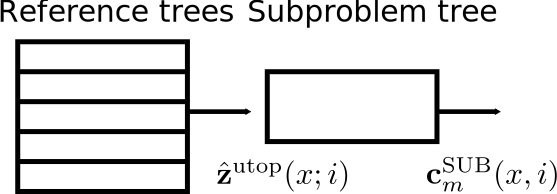
\includegraphics[width=0.5\linewidth]{fig/cascade}
\caption{The dependency of the trees in MORRF$^{*}$.}
\label{fig:dependency}
\end{figure}

\begin{asmp}{(Continuity of the objective functions)}
\label{asmp:continuity}
For all $k\in K$, the cost function $c_{k}$ is Lipshitz continuous, that is, for all paths $\sigma_1 : [0, s_{1}] \rightarrow X_{\it free}$ and $ \sigma_2 : [0, s_{2}] \rightarrow X_{\it free}$, there exists a (cost function dependent) constant $\kappa(k)\in \mathbb{R}_{+}\cup \{0 \}$ such that $ | c_{k} ( \sigma_{1} ) - c_{k} ( \sigma_{2} ) | \leq \kappa(k) \sup_{\tau \in [0, 1]} \lVert \sigma_{1} (\tau s_{1}) - \sigma_{2} (\tau s_{2}) \rVert $.
\end{asmp}


\begin{asmp}{(Obstacle spacing)}
\label{asmp:spacing}
There exists a constant $ \delta \in \mathbb{R}_{+} $ such that $ \forall x \in X_{\it free} $ , $ \exists x' \in X_{\it free} $ such that
\begin{itemize}
\item the $ \delta $-ball centered at $ x' $ lies inside $ X_{\it free} $;
\item $ x $ lies inside the $ \delta $-ball centered at $ x' $.
\end{itemize}
\end{asmp}


\begin{lem}
\label{lem:sol_pareto_opt}
If the Utopia vector satisfies $\forall k,\sigma\  z_k^{\rm utop}\leq c_{k}( \sigma)$, then any solution of Eq.~ \eqref{eq:Tchebycheff} is Pareto optimal.
\begin{proof}
The proof is by contradiction.  
Let the weighting vector ${\mathbf \lambda}$ be arbitrary subject to $\forall k\ \lambda_k\geq 0$, and let $ \sigma^*=\sigma^{*}({\mathbf \lambda}) $ be a solution given that weighting vector. 
By definition, 
\begin{equation}
\label{eq:tchebycheff:argmin}
\sigma^{*} = \arg \min_{ \sigma } \max_{ k \in K }  \lambda_{k} | c_{k}( \sigma ) - z^{\rm utop}_{k} | .
\end{equation}
Assume that the path $ \sigma^{*} $ is not Pareto optimal.
Then there exist another path $ \sigma^{o} $ that dominates $ \sigma^{*} $
%, meaning
%\begin{eqnarray}
%\nonumber
%\forall k \in K , & c_{k}( \sigma^{o} ) \leq c_{k}( \sigma^{*} ); \\
%\nonumber
%\exists k' \in K , & c_{k'}( \sigma^{o} ) < c_{k'}( \sigma^{*} ).
%\end{eqnarray}
%Because the Utopia reference vector satisfies, 
and the Utopia reference vector that satisfies
$ \forall k \in K $, $ z^{\rm utop}_{k} \leq  c_{k}( \sigma ) $, it follows that
\begin{eqnarray}
\nonumber
\forall k \in K , & z^{\rm utop}_{k} \leq c_{k}( \sigma^{o} ) \leq c_{k}( \sigma^{*} ) ; \\
\nonumber
\exists k' \in K , & z^{\rm utop}_{k} \leq c_{k'}( \sigma^{o} ) < c_{k'}( \sigma^{*} ).
\end{eqnarray}
These equations imply
\begin{eqnarray}
%\nonumber
%\forall k \in K , & c_{k}( \sigma^{*} ) - z^{\rm utop}_{k} \geq c_{k}( \sigma^{o} ) - z^{\rm utop}_{k} \geq 0 ; \\
%\nonumber
%\exists k' \in K , &  c_{k'}( \sigma^{*} ) - z^{\rm utop}_{k} > c_{k'}( \sigma^{o} ) - z^{\rm utop}_{k} \geq 0 ;\\
\nonumber
\forall k \in K , & \lambda_{k} | c_{k}( \sigma^{*} ) - z^{\rm utop}_{k} | \geq \lambda_{k}  | c_{k}( \sigma^{o} ) - z^{\rm utop}_{k} | ; \\
\nonumber
\exists k' \in K , & \lambda_{k'}  | c_{k'}( \sigma^{*} ) - z^{\rm utop}_{k} | > \lambda_{k'}  | c_{k'}( \sigma^{o} ) - z^{\rm utop}_{k} | ;
\end{eqnarray}
which yields the following contradiction to Eq~\eqref{eq:tchebycheff:argmin}:
\begin{equation}
\nonumber
\max_{ k \in K }  \lambda_{k} | c_{k}( \sigma^{*} ) - z^{\rm utop}_{k} | > \max_{ k \in K } \lambda_{k}  | c_{k}( \sigma^{o} ) - z^{\rm utop}_{k} |.
\end{equation}
%which contradicts with Equation \eqref{eq:tchebycheff:argmin}.
\end{proof}
\end{lem}

%Before presenting the following lemma and proof, note that we modify the definition of the Utopia vector to satisfy a technical requirement: 
%$z_k^{\rm utop} = \inf_{\sigma\in X_{\rm free}} c_{k}(\sigma) - \delta$ for $\delta$ some small real number.
\begin{lem}
\label{lem:exist_weight}
If $ \sigma^{*} $ is Pareto optimal then there exists a weighting vector $ \bm{\lambda} $, where $ \forall k \ \lambda_k\geq 0$ and $\sum_{k=1}^{K} \lambda_{k} = 1 $, such that $ \sigma^{*} $ is a solution of Eq.~\eqref{eq:Tchebycheff}.
\begin{proof}
This is a proof by construction over cases.  
When $ \sigma^{*} $ is Pareto optimal, there exist two cases: (a)~$ \exists k ,  c_{k}( \sigma ) = z^{\rm utop}_{k} $ and (b)~$ \forall k,  c_{k}( \sigma^{*} ) < z^{\rm utop}_{k} $.

%\begin{itemize}
\textit{\textbf{Case (a):}} $ \exists k ,  c_{k}( \sigma ) = z^{\rm utop}_{k} $ \\
Define $ P(\sigma^*)=\{ j \ \mid  c_{j}(\sigma^*)=z_j^{\rm utop}\} $ and let $ \overline{P}=\{1,\ldots,K\} \setminus P $.
%Let the cardinality of $ P(\sigma^*) $ be $ len(P(\sigma^*)) $.
Define the weight vector $ \bm{\lambda} $ as 
\begin{equation}
  \lambda_k = \left\{
    \begin{array}{cc}
      \frac{1}{|P|} & k\in P(\sigma^*) \\
      0 & k\in\overline{P}(\sigma^*)
    \end{array}\right..
\end{equation}
%\begin{itemize}
	%\item $ \forall k \in P(\sigma^*), \lambda_{k} = 1 / len(P(\sigma^*)) $;
	%\item $ \forall k \in \overline{P}(\sigma^*), \lambda_{k} = 0 $.
%\end{itemize}
For these weights, Eq.~\eqref{eq:Tchebycheff} returns a set of solution paths, all of which have the same cost for the $k$-cost functions when $k\in P$ but different possible costs for $k\in\overline{P}$.  $\sigma^*$ is trivially in this set of solution paths.

\textit{\textbf{Case (b)}}: $\forall k,  c_{k}( \sigma^{*} ) > z^{\rm utop}_{k}$\\
For all $k$, define the weights as
%\begin{equation}
%\label{eq:weights:assign}
%\forall k \in K, 
$\lambda_{k} = \frac{ \ell_{k} }{ \sum_{j=1}^K \ell_{j} }$, where
%\end{equation}
$ \ell_{k} =\frac{1}{| c_{k}(\sigma^*)-z^{\rm utop}_{k} |} $.
The Tchebycheff cost (Eq.~\eqref{eq:Tchebycheff}) becomes
\begin{equation}
\nonumber
\begin{aligned}
	g^{te} ( \sigma^{*} ) %=& \max_{k \in K} \lambda_{k} | c_{k}( \sigma^* ) - z^{\rm utop}_{k} | \\
	%=& \max_{k\in K} \frac{\ell_k}{\sum_{j=1}^{K} \ell_j}  | c_{k}( \sigma^* ) - z^{\rm utop}_{k} | \\
	= \max_{k \in K}  \frac{| c_{k}( \sigma^* ) - z^{\rm utop}_{k} |}{ | c_{k}( \sigma^* ) - z^{\rm utop}_{k} |} \frac{1}{\sum_{j=1}^K \ell_j} 
	= \frac{1}{\sum_{j=1}^K \ell_j} \\
\end{aligned}
\end{equation}
%
Given any other path $ \sigma $, we can represent the Tchebycheff cost as follows:
%\begin{equation}
\begin{eqnarray*}
%\label{eq:exist_weight:leq}
%\begin{aligned}
 g^{te} ( \sigma )%& = &
 %\max_{k \in K} \lambda_{k} | c_{k}( \sigma ) - z^{\rm utop}_{k} | \\
 &=& \max_{k\in K} \frac{ \ell_{k} }{ \sum_{j=1}^K \ell_{j} } | c_{k}( \sigma ) - z^{\rm utop}_{k} | \\
% &= & \frac{1}{\sum_{j=1}^K \ell_j}\max_{k \in K} \frac{ | c_{k}( \sigma ) - z^{\rm utop}_{k} |  }{ | c_{k} ( \sigma^{*} ) - z^{\rm utop}_{k} | } \\%\left( \sum_{j=1}^K \ell_{j}  \right)^{-1} \\
 %&= & \left( \sum_{j=1}^K \ell_{j}  \right)^{-1} \max_{k \in K} \left| \frac{ c_{k}( \sigma ) - z^{\rm utop}_{k}  }{ c_{k} ( \sigma^{*} ) - z^{\rm utop}_{k} } \right| \\
% &= & \frac{1}{\sum_{j=1}^K \ell_j}\max_{k \in K} \left| \frac{ c_{k}( \sigma ) - c_{k} ( \sigma^{*} )  +  c_{k} ( \sigma^{*} ) - z^{\rm utop}_{k}  }{  c_{k} ( \sigma^{*} ) - z^{\rm utop}_{k} } \right| \\
 &= & \frac{1}{\sum_{j=1}^K \ell_j} \max_{k \in K} \left| 1 + \frac{ c_{k}( \sigma ) - c_{k} ( \sigma^{*} )  }{  c_{k} ( \sigma^{*} ) - z^{\rm utop}_{k} } \right|
%\end{aligned}
%\end{equation}
\end{eqnarray*}
%
Because $ \sigma^{*} $ is Pareto optimal,
%\begin{equation}
%\label{eq:exist_geq}
$\exists k' \in K, c_{k'} ( \sigma ) >  c_{k'} ( \sigma^{*} )$.
%\end{equation}
As $ \forall k,  c_{k}( \sigma^{*} ) > z^{\rm utop}_{k} $,
we have $ \forall k,  c_{k}( \sigma^{*} ) - z^{\rm utop}_{k} > 0 $.
This implies
%\begin{equation}
%\exists k' \in K, 
$\frac{ c_{k'}( \sigma ) - c_{k'} ( \sigma^{*} )  }{  c_{k'} ( \sigma^{*} ) - z^{\rm utop}_{k'} }  > 0$,
%\end{equation}
which, in turn, implies that
%\begin{equation}
$
\max_{k \in K} \left| 1 + \frac{ c_{k}( \sigma ) - c_{k} ( \sigma^{*} )  }{  c_{k} ( \sigma^{*} ) - z^{\rm utop}_{k} } \right| > 1.
$ %\end{equation}
Therefore,
%\begin{equation}
%\begin{aligned}
$
g^{te} ( \sigma ) >  \frac{1}{\sum_{j=1}^K \ell_j} = g^{te} ( \sigma^{*} )$.
%\end{aligned}
%\end{equation}
%It means,
%\begin{equation}
%\forall \sigma, g^{te} ( \sigma ) > g^{te} ( \sigma^{*} ).
%\end{equation}
Thus, $  \sigma^{*} $ is a solution to Eq. \eqref{eq:Tchebycheff}.

\end{proof}
\end{lem}

By Lemma \ref{lem:sol_pareto_opt} and Lemma \ref{lem:exist_weight}, we have the following:

\begin{thm}
\label{thm:moo-d:rrt}
A path is Pareto optimal if and only if it is a solution to Eq.~\eqref{eq:Tchebycheff} for some weight vector.
%\begin{proof}
%By Lemma \ref{lem:sol_pareto_opt}, we know that each solution to Equation \eqref{eq:Tchebycheff} is a solution in Pareto optimal set.
%By Lemma \ref{lem:exist_weight}, we know that each solution in Pareto optimal set, there exits a weight that makes the solution an answer to Equation \eqref{eq:Tchebycheff}.
%Thus, we know that the Pareto optimal set $ \{ \sigma^{*} \} $ is the range of the function value defined by Equation %\eqref{eq:Tchebycheff}.
%\end{proof}
\end{thm}


Theorem~\ref{thm:moo-d:rrt} implies that we can use the Tchebycheff method to find the Pareto set for the multi-objective path-planning problems.  
In terms of the MORRF$^{*}$ algorithm, we can sample the Pareto set by selecting weights, forming a subproblem that can be solved using RRT$^{*}$. 
The next question that needs to be answered is whether the subproblem tree can find the optimal solution of its assigned subproblem.

The way that the RRT$^{*}$ algorithm works is that it incrementally constructs a tree from a root position.  
New nodes are constructed by randomly sampling points that are near to other locations in the tree, and then wiring the new node and rewiring nearby nodes in the tree so that the path from root to the position of the new node is minimal.  
The cost of the path from the position of the root node to the positions of every other node converges to the minimal possible cost between the positions as the number of iterations approaches infinity.  
We restate this as a lemma, and note that the corresponds exactly to that given for Theorem 22 in~\cite{Karaman.Frazzoli:RSS10}.
\begin{lem}
\label{lem:tree_vex:conv}
Given Assumptions~\ref{asmp:additivity}-\ref{asmp:spacing},
the cost of the minimum cost path from the root to any vertex in RRT$^{*}$ converges to the optimal cost almost surely.
\end{lem}
  
\begin{comment}
Let $c(x; i) $ be the minimum cost from the root to the position of vertex $ x $ at iteration $ i$  and $ z^{*}(x) $ be the minimum cost from the start to the position of vertex $ x $.
We can generalize the conclusion of Theorem 22 in \cite{Karaman.Frazzoli:RSS10} to all the vertices in the RRT$^{*}$.
\begin{lem}
%\label{lem:tree_vex:conv}
Given Assumptions~\ref{asmp:additivity}-\ref{asmp:spacing},
the cost of the minimum cost path from the root to any vertex in RRT$^{*}$ converges to the optimal cost almost surely, i.e.,
$
P( \{ \lim_{ i \rightarrow \infty } c(x, i)  = z^{*}(x) \} ) = 1, x \in V $.
\begin{proof}
%The construction of RRT* is not goal-oriented.
%The ``rewire'' process potentially will update all the vertices and converge the value to the optimal one.
%Similar with that of a goal vertex, the paths from the root to all other vertices will converge to corresponding optimal ones as well.
The asymptotic optimality of RRT$^{*}$ does not rely on how the sampling process is like (Theorem 22, \cite{Karaman.Frazzoli:RSS10}), though the convergence rate might be different.
Simply changing the goal to the position of any vertex still hold the asymptotic optimality.
Thus, we could generalize the asymptotic optimality from the goal to all the vertices.
\end{proof}
\end{lem}
\end{comment}

Lemma~\ref{lem:tree_vex:conv} and Theorem~\ref{thm:moo-d:rrt} imply that each reference tree converges to the optimal path from the root to any node in the tree, including a node arbitrarily close to the goal node.  
This means that the costs returned by those trees for the path from start to goal for cost function $c_k$ converges to the $k^{\rm th}$ element of the Utopia reference vector $ \bm{z}^{\rm utop} $.  
We state this as a lemma.
\begin{lem}
\label{lem:ref_tree:conv}
Given Assumptions \ref{asmp:additivity}-\ref{asmp:spacing},
the cost of the minimum cost path from the root to any vertex in $ k^{\rm th} $ reference tree converges to $ z^{*}_{k} $ almost surely. %, i.e., 
%$ P( \{ \lim_{ i \rightarrow \infty }  c^{\rm REF}_{k} (x, i) = z^{*}_{k} (x) \} ) = 1  $.
\end{lem}

We now turn to the proof that the subproblem trees converge to paths in the Pareto set.
The proof of this claim is that we need to know $\bm{z}^{\rm utop} $ to compute the Tchebycheff cost associated with the cost used in the subproblem. 
If we knew that the reference trees had already converged to $\bm{z}^{\rm utop} $, then we could simply instantiate Lemma~\ref{lem:tree_vex:conv}, but the problem is that reference trees are converging at the same time that the subproblem trees are converging.
We now address this problem.  

Let $ \hat{\bm{z}}^{\rm utop}(v;i) $ denote the approximate Utopia reference vector for position $v$ on iteration $i$, obtained by looking the cost from the root to position $x$ from the $k$-reference trees.
Recall that the $m^{\rm th}$ subtree attempts to generate a solution to Eq.~\eqref{eq:Tchebycheff} for a given weight vector ${\mathbf \lambda}^m$.
Let
\begin{equation}
\label{eq:c_def}
 \bm{c}^{\rm SUB}_{m} ( \bm{z} ) 
 = \arg \min_{x} \max_{ k \in K } \lambda_{m, k} | x_{k} - \bm{z}_{k} | 
\end{equation} denote the as the cost vector in $ m^{\rm th} $ subproblem tree given the reference vector $ \bm{z} $.
$ \hat{ \bm{c} }^{\rm SUB}_{m} ( i, \bm{z} ) $ as its estimation at iteration $ i $.
A subproblem tree obtains $ \hat{\bm{z}}^{\rm utop} (v) $ for vertex $ v $ from the reference trees and generate the corresponding $ \bm{c}^{\rm SUB}_{m} ( v ; i, \hat{\bm{z}}^{\rm utop} (v) ) $ at iteration $ i $ for either adding new vertex or rewiring an existing vertex.
This forms a cascade structure from the reference trees to the subproblem tree. 
By Lemma \ref{lem:ref_tree:conv}, we have the convergence of the reference trees.

\begin{asmp}{(Lipschitz continuity)}
\label{asmp:lipschitz}
$ \bm{c}^{\rm SUB}_{m} ( \bm{z} )  $ in Eq. \eqref{eq:c_def} is Lipschitz continuity, i.e.
$ \lVert \bm{c}^{\rm SUB}_{m} ( \bm{z}_{a} ) - \bm{c}^{\rm SUB}_{m} ( \bm{z}_{b} ) \rVert \leq K \lVert \bm{z}_{a} - \bm{z}_{b} \rVert $.
\end{asmp}

\begin{lem}
\label{lem:sub_tree:conv}
Given Assumptions~\ref{asmp:additivity}-\ref{asmp:lipschitz} and given the estimated Utopia reference vector $ \hat{\bm{z}} $,
%with $ \bm{z}^{\rm utop} (x) $ for any $ x $ given,
the cost of the solution of $ m^{\rm th} $ subproblem tree converges to the corresponding cost of the $ m^{\rm th} $ subproblem $ \bm{c}_{m}^{*} ( \hat{\bm{z}} ) $ almost surely.
\end{lem}

\begin{comment}
\begin{lem}
\label{lem:morrf:conv}
Given Assumptions~\ref{asmp:additivity}-\ref{asmp:lipschitz} and given the correct value of the Utopia reference vector,
%with $ \bm{z}^{\rm utop} (x) $ for any $ x $ given,
the cost of the solution of $ m^{\rm th} $ subproblem tree converges to the optimal cost of the $ m^{\rm th} $ subproblem almost surely, i.e.,
\begin{equation}
\label{eq:sub_tree:conv}
P( \{ \lim_{ \substack{ i \to \infty \\ j \to \infty } } \bm{c}^{\rm SUB}_{m} (i , \hat{\bm{z}} (j) ) =  \bm{c}_{m}^{*}  \} ) = 1 .
\end{equation}
\end{lem}
\end{comment}

Now, we can prove that the solutions from MORRF$^{*}$ almost surely converges to a subset of the Pareto optimal set.

\begin{thm}
\label{thm:morrt:conv}
When Assumption \ref{asmp:additivity}, \ref{asmp:continuity} and \ref{asmp:spacing} hold,
the solutions from MORRF$^{*} $ converges to a subset of the Pareto optimal set almost surely, i.e.
$
P( \lim_{ i \to \infty }  \Sigma^{\mbox{MORRF}^{*}}_{i}  \subset \Sigma^{*} ) = 1.
$
%\begin{proof}
%As the solutions of MORRF$^{*}$ can be modeled in points in a high-dimension space by Lemma \ref{lem:moo-d:rrt}, the %Tchebycheff method could be imported to decompose the multi-objective optimization problem into a set of subproblems.
%By the fitness definition of the subproblem trees, if the subproblem tree could find a solution that minimize the fitness, the %solution is in the Pareto optimal set of the multi-objective optimization problem.
%
%Lemma \ref{lem:ref_tree:conv} guarantees that the reference vector $ \bm{z}^{\rm utop}(x) $ at any location $ x $ %converges to the correct estimation after running enough iteration.
%Thus, by Lemma \ref{lem:sub_tree:conv}, we have that the solution cost of the $ m $-th subproblem tree converges to $ %z^{*}_{ \lambda_{m} } $.
%It means that the solution converges to an optimal solution to $ m $-th subproblem as the iteration goes.
%Therefore, the set of the solutions from all the subproblem trees converge to a subset of the Pareto optimal set, as the %iteration goes~\cite{4358754}~\cite{miettinen1999nonlinear}.
%\end{proof}
\end{thm}

\section{Simulation}
\label{sec:simulation}

\begin{comment}
2D (weighted sum + Tchebycheff method)
2D (With obstacles)
3D
compare NSGA-II
\end{comment}

We now present a series of simulation studies that provide evidence that MORFF$^{*}$ produces a representative set of samples from the Pareto set.
Results from MORFF$^{*}$ are obtained for path-planning problems with two objectives and three objectives, and are compared to a modified version of the NSGA-II multi-objective path-planning algorithm~\cite{Ahmed2013} as well as a variant of MORFF$^{*}$ that uses a weighted sum rather than the Tchebycheff approach.
NSGA-II was selected because evidence suggests that it provides more uniform samples from the Pareto set than other approaches~\cite{deb2002fast}.  
We modified the NSGA-II algorithm for this problem to use paths as inputs, represented by a series of waypoints connected by line segments;he cost calculation is identical with that in  MORRF$^{*}$, calling \textsc{Line}($ x_{1}, x_{2} $) to calculate the cost between two way points $ x_{1} $ and $ x_{2} $.  
The weighted sum approach was chosen because evidence suggests that it works well only when all the objectives are convex~\cite{4358754} whereas the Tchebycheff approach should bring better diversity in the solutions~\cite{4358754}.  
The weighted sum approach uses the same sampling method for weights as that used to generate the $\lambda_i$ in MORFF$^{*}$.
Each method was run for $ 5000 $ iterations and restricted to $ 30 $ solutions.  

The first simulation study compares there three algorithms in an obstacle-free world with two objectives: 
minimize Euclidean distance, see Figure~\ref{fig:sim:norm:distance}, and minimize a cost function, see Figure~\ref{fig:sim:norm:fitness1}, which has dark colors as low costs and light colors as high costs.  


The first thing to note is that the convergence of NSGA-II-based path-planning is very slow.
This is indicated in Figures~\ref{fig:sim:norm:pf:a}-\ref{fig:sim:norm:sols:a}, which show the approximation to the Pareto set and corresponding paths, respectively, after $5000$ iterations; observe how the quality of the paths and sampling of the Pareto set is uneven and unsatisfactory.
By contrast, the weighted sum approach returns a set of high-quality solutions close to the Pareto optimal set, see Figures~\ref{fig:sim:norm:pf:b} and \ref{fig:sim:norm:sols:b}; especially note the difference in x-axis values (corresponding to the costs of the paths) between the solutions from NSGA-II and the MORFF$^{*}$ using weighted sum.
Finally, note the somewhat uneven clustering of solutions on Pareto front for MORFF$^{*}$ using weighted sum, and compare this to the slightly more uniform clustering of MORFF$^{*}$ using the Tchebycheff approach in Figures~\ref{fig:sim:norm:pf:c}-\ref{fig:sim:norm:sols:c}.

\begin{figure}[h!]
	\centering
	\begin{subfigure}[b]{0.35\linewidth}
		\centering
		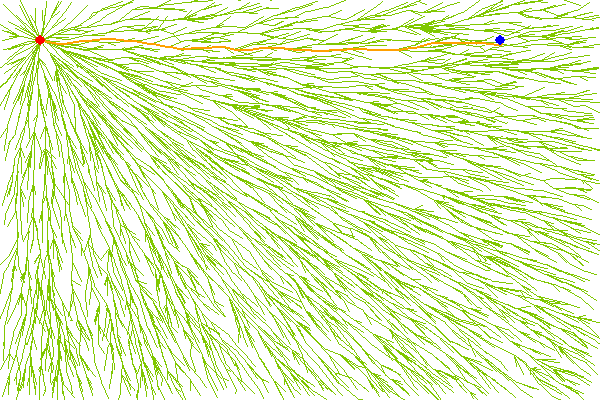
\includegraphics[width=\textwidth]{fig/sim2-2obj/MORRTstar00-0.png}
		\caption{Minimize distance}
		\label{fig:sim:norm:distance}
	\end{subfigure}
	\begin{subfigure}[b]{0.35\linewidth}
		\centering
		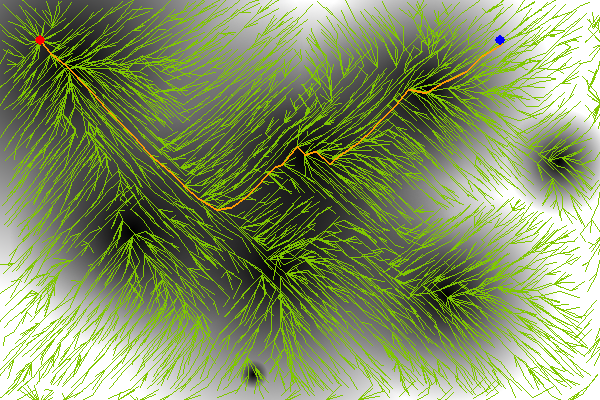
\includegraphics[width=\textwidth]{fig/sim2-2obj/MORRTstar00-1.png}
		\caption{Minimize cost 1}
		\label{fig:sim:norm:fitness1}
	\end{subfigure}  \\
	\begin{subfigure}[b]{0.31\linewidth}
		\centering
		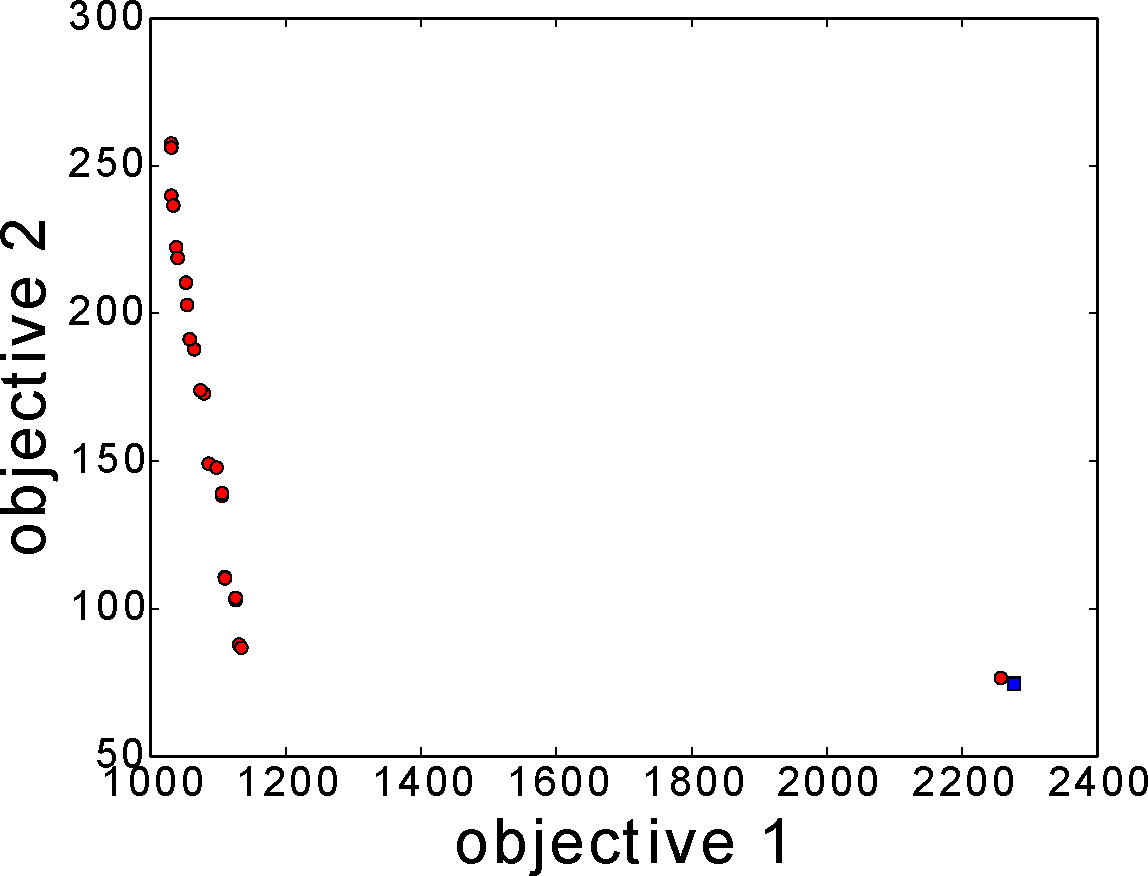
\includegraphics[width=\textwidth]{fig/sim3-2obj/PF03-MOPATH.pdf}
		\caption{Pareto set: NSGA-II}
		\label{fig:sim:norm:pf:a}
	\end{subfigure}
	\begin{subfigure}[b]{0.31\linewidth}
		\centering
		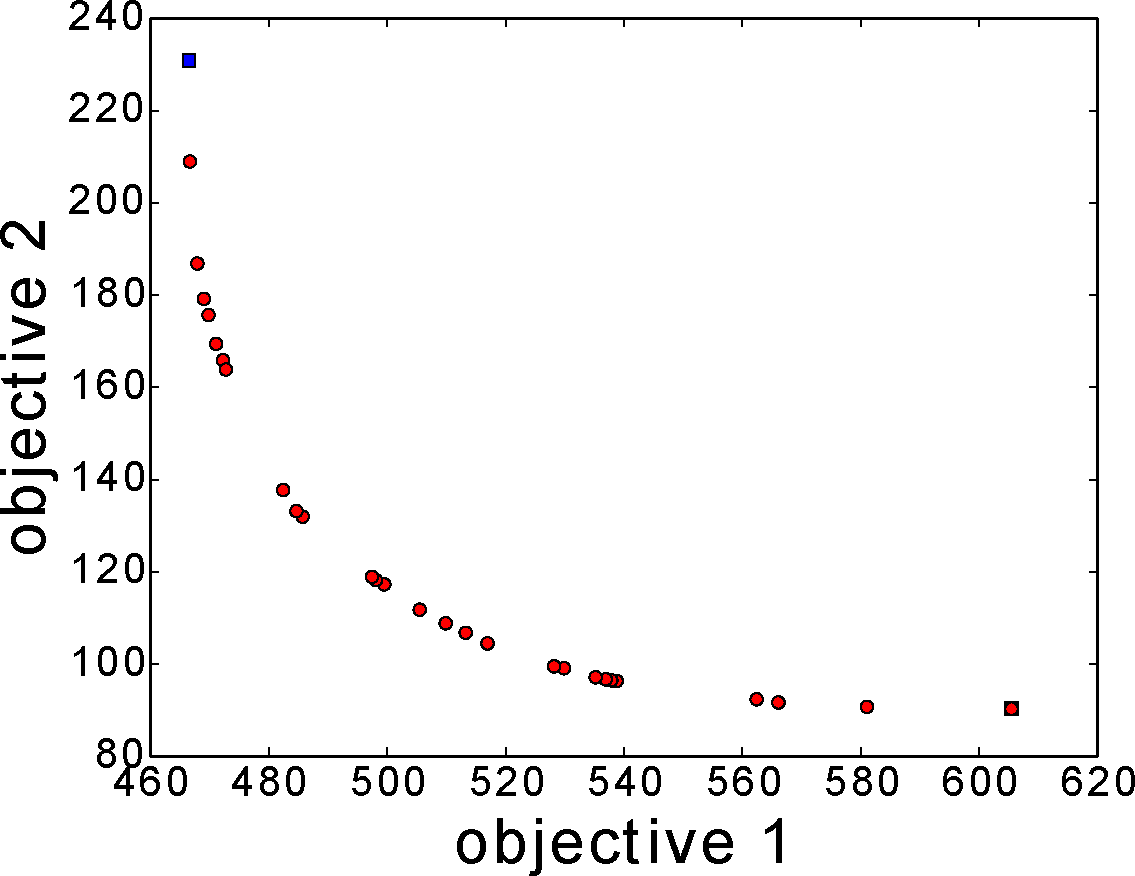
\includegraphics[width=\textwidth]{fig/sim1-2obj/PF01-MORRT.pdf}
		\caption{Pareto set: weighted sum}
		\label{fig:sim:norm:pf:b}
	\end{subfigure}
	\begin{subfigure}[b]{0.31\linewidth}
		\centering
		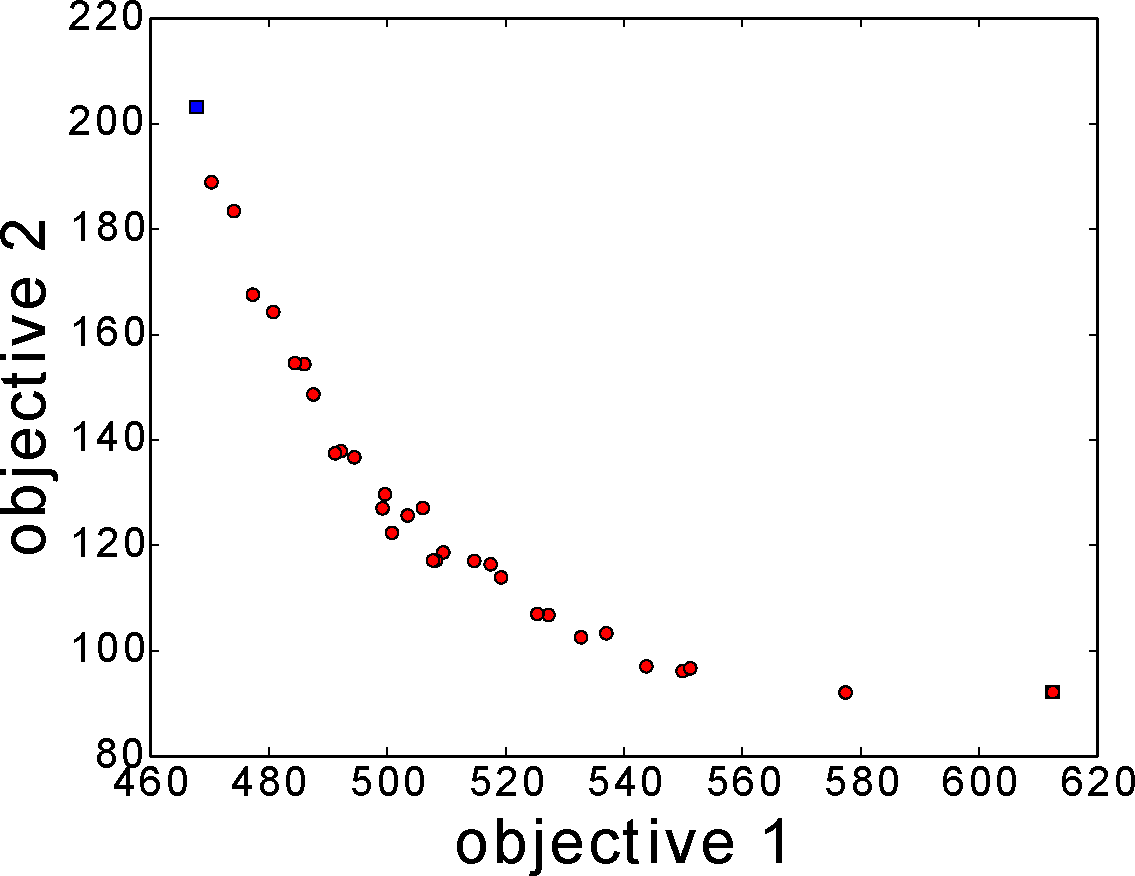
\includegraphics[width=\textwidth]{fig/sim2-2obj/PF02-MORRT2.pdf}
		\caption{Pareto set: Tchebycheff}
		\label{fig:sim:norm:pf:c}
	\end{subfigure}  \\
	\begin{subfigure}[b]{0.31\linewidth}
		\centering
		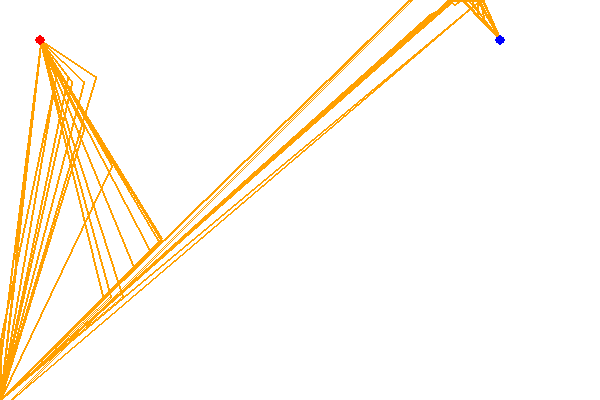
\includegraphics[width=\textwidth]{fig/sim3-2obj/MOPath01-ALL.png}
		\caption{Pareto paths: NSGA-II}
		\label{fig:sim:norm:sols:a}
	\end{subfigure} 
	\begin{subfigure}[b]{0.31\linewidth}
		\centering
		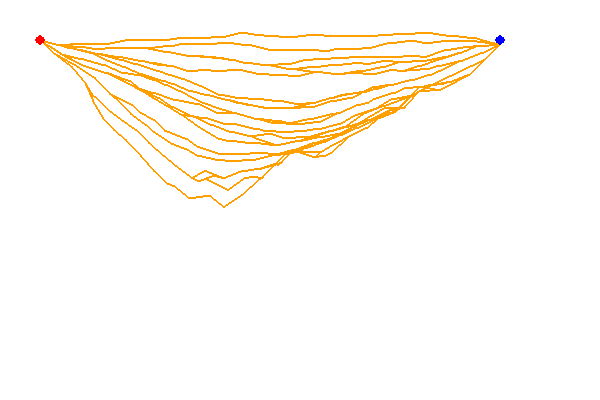
\includegraphics[width=\textwidth]{fig/sim1-2obj/MORRTstar00-ALL.png}
		\caption{Pareto paths: weighted sum}
		\label{fig:sim:norm:sols:b}
	\end{subfigure} 
	\begin{subfigure}[b]{0.35\linewidth}
		\centering
		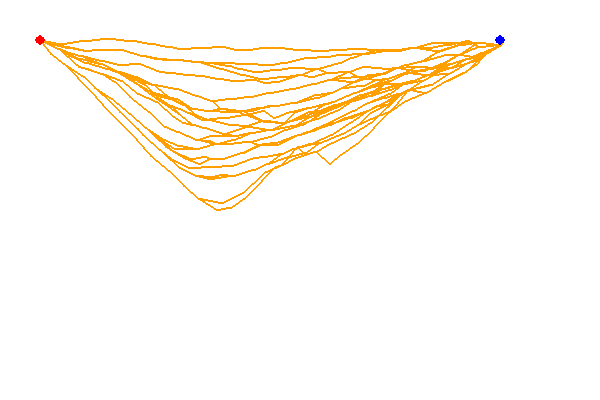
\includegraphics[width=\textwidth]{fig/sim2-2obj/MORRTstar00-ALL.png}
		\caption{Pareto paths: Tchebycheff}
		\label{fig:sim:norm:sols:c}
	\end{subfigure}
	\caption{Path planning with two objectives.}
	\label{fig:sim:norm}
\end{figure}

Recall that the weighted sum approach is designed to work well for convex sets and the Tchebycheff approach is designed to give more uniform sampling for non-convex sets. 
We therefore compared results for the two approaches for an environment with obstacles, omitting results for NSGA-II because convergence is so slow.  
The results are shown in Figure \ref{fig:sim:obs}.
As before, observe that the Tchebycheff approach yields a more uniform sampling, albeit one that appears to be somewhat noisy approximation to the Pareto set.

\begin{figure}[h!]
	\centering
	\begin{subfigure}[b]{0.35\linewidth}
		\centering
		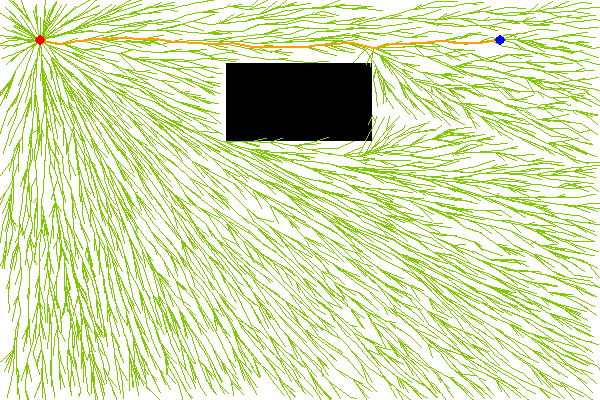
\includegraphics[width=\textwidth]{fig/sim4-obstacle/MORRTstar01-1-0.png}
		\caption{Minimize distance}
		\label{fig:sim:obs:distance}
	\end{subfigure}
	\begin{subfigure}[b]{0.35\linewidth}
		\centering
		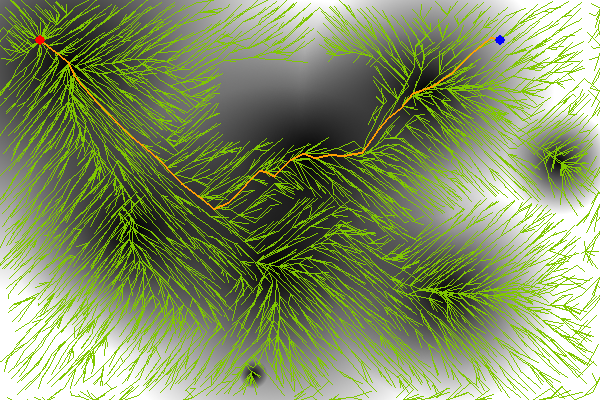
\includegraphics[width=\textwidth]{fig/sim4-obstacle/MORRTstar01-1-1.png}
		\caption{Minimize cost 1}
		\label{fig:sim:obs:fitness1}
	\end{subfigure}  \\
	\begin{subfigure}[b]{0.35\linewidth}
		\centering
		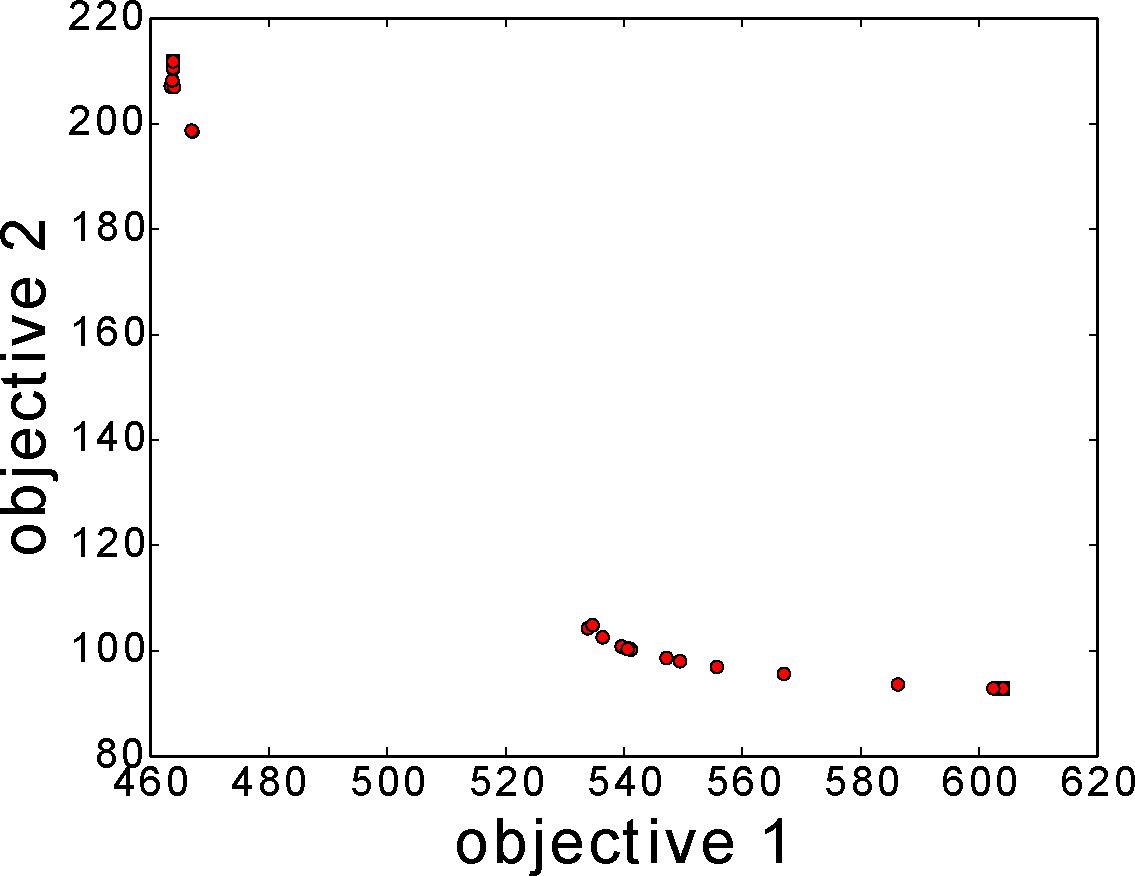
\includegraphics[width=\textwidth]{fig/sim4-obstacle/PF04-MORRT.pdf}
		\caption{Paretoset: weighted sum}
		\label{fig:sim:obs:pf:a}
	\end{subfigure}
	%\begin{subfigure}[b]{0.35\linewidth}
	%	\centering
	%	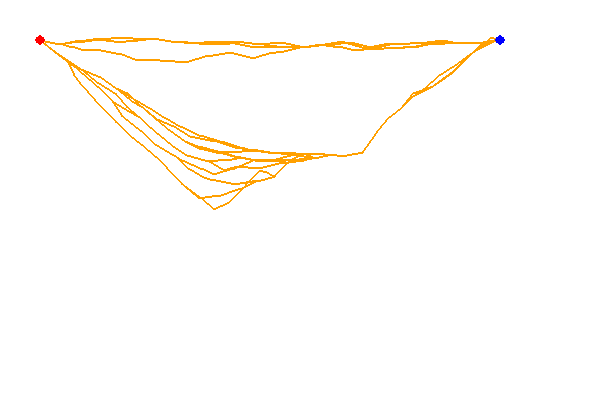
\includegraphics[width=\textwidth]{fig/sim4-obstacle/MORRTstar01-1-ALL.png}
	%	\caption{Pareto paths: weighted sum}
	%	\label{fig:sim:obs:sols:a}
	%\end{subfigure}  \\
	\begin{subfigure}[b]{0.35\linewidth}
		\centering
		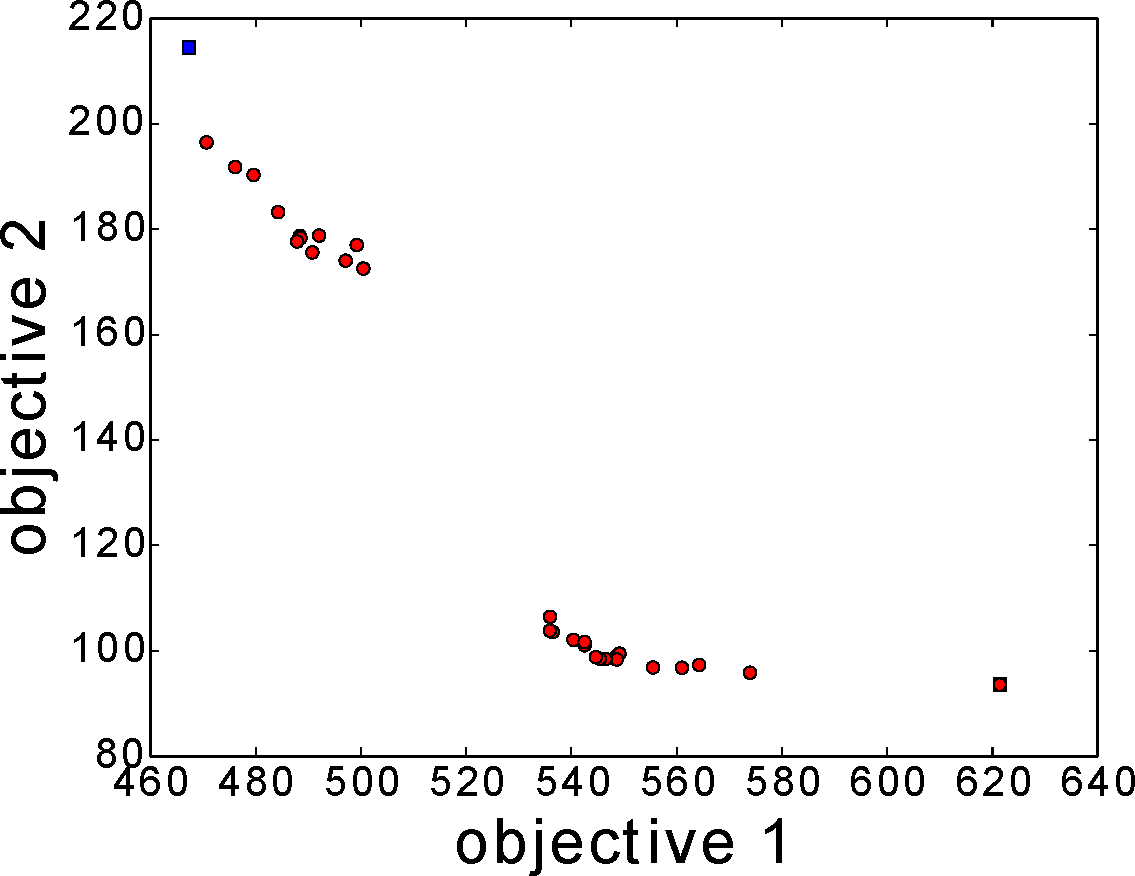
\includegraphics[width=\textwidth]{fig/sim5-obstacle/PF05-MORRT2.pdf}
		\caption{Pareto set: Tchebycheff}
		\label{fig:sim:obs:pf:b}
	\end{subfigure} 
	%\begin{subfigure}[b]{0.35\linewidth}
	%	\centering
	%	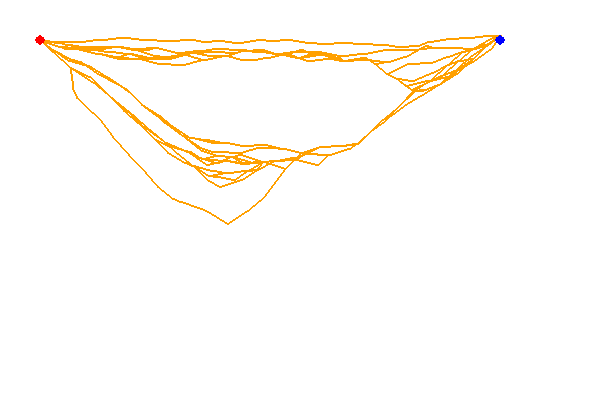
\includegraphics[width=\textwidth]{fig/sim5-obstacle/MORRTstar01-1-ALL.png}
	%	\caption{Pareto paths: Tchebycheff}
	%	\label{fig:sim:obs:sols:b}
	%\end{subfigure}
	\caption{Path planning with two objectives and an obstacle.}
	\label{fig:sim:obs}
\end{figure}

\begin{comment}
We then tested the MORFF$^{*}$ algorithms on a two-objective problem  in which there exists a conflict in the costs; 
see Figures~\ref{fig:sim:nonconvex:fitness1}-\ref{fig:sim:nonconvex:fitness2}. 
The results illustrated in Figure~\ref{fig:sim:nonconvex} illustrate that, once again, the Tchebycheff approach shows better diversity but is somewhat more noisy than the weighted sum approach in Figure \ref{fig:sim:nonconvex}.

\begin{figure}
	\centering
	\begin{subfigure}[b]{0.45\linewidth}
		\centering
		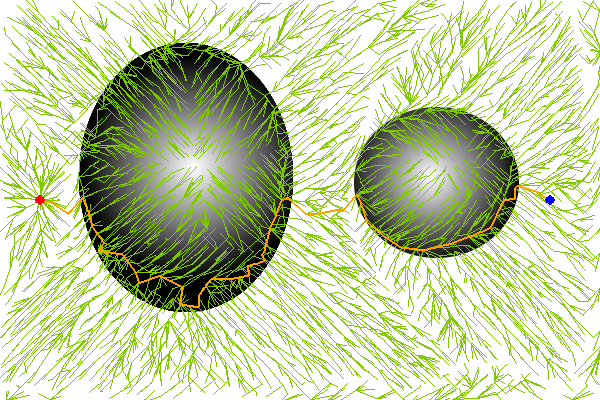
\includegraphics[width=\textwidth]{fig/sim8-nconvex/MORRTstar03-0.png}
		\caption{Minimize cost 1}
		\label{fig:sim:nonconvex:fitness1}
	\end{subfigure}
	\begin{subfigure}[b]{0.45\linewidth}
		\centering
		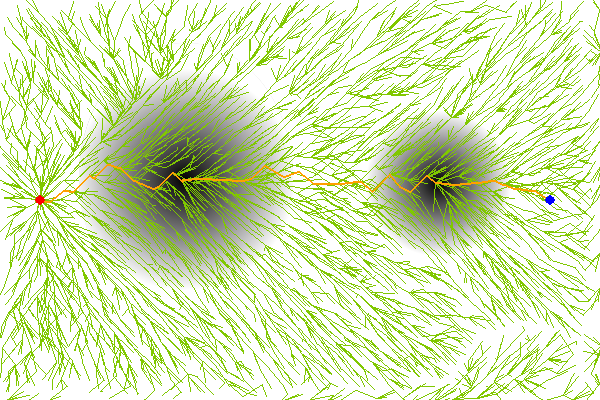
\includegraphics[width=\textwidth]{fig/sim8-nconvex/MORRTstar03-1.png}
		\caption{Minimize cost 2}
		\label{fig:sim:nonconvex:fitness2}
	\end{subfigure}  \\
	\begin{subfigure}[b]{0.45\linewidth}
		\centering
		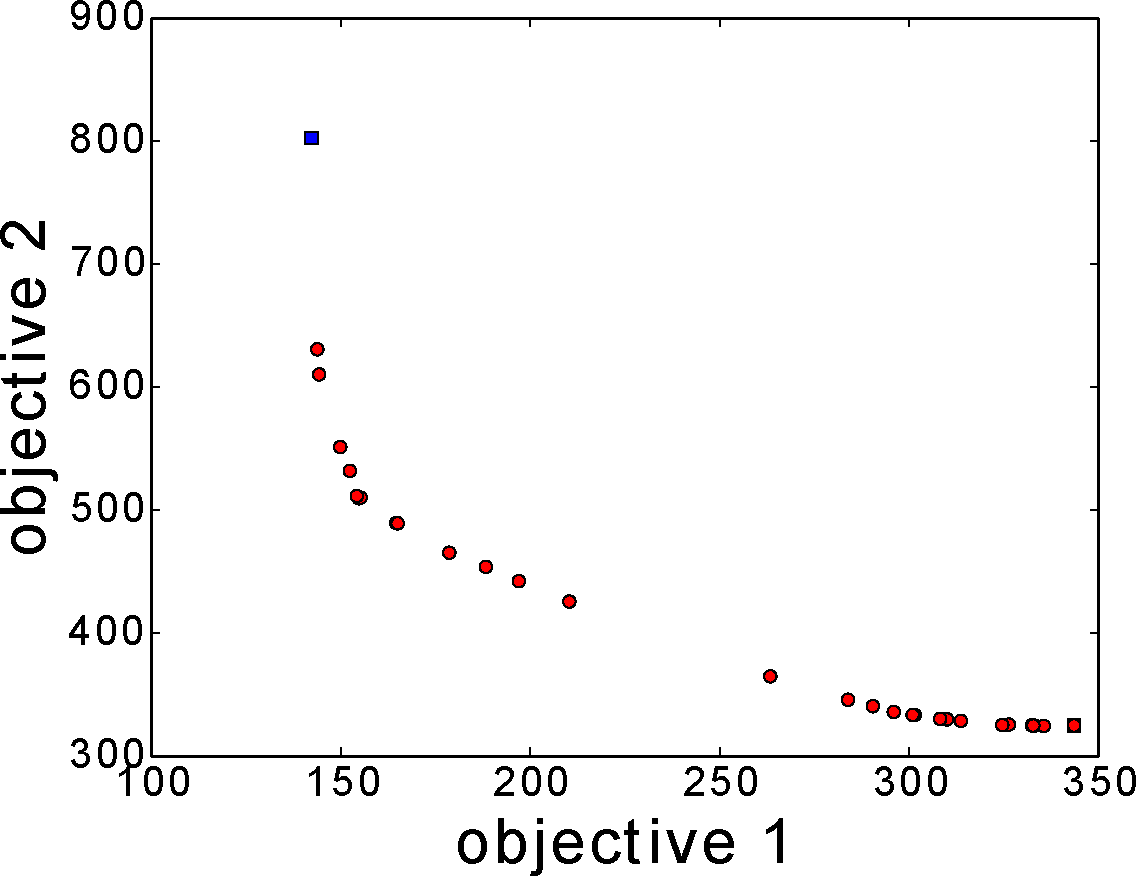
\includegraphics[width=\textwidth]{fig/sim8-nconvex/PF03-MORRT.pdf}
		\caption{Pareto set: weighted sum}
		\label{fig:sim:nonconvex:pf:a}
	\end{subfigure}
	\begin{subfigure}[b]{0.45\linewidth}
		\centering
		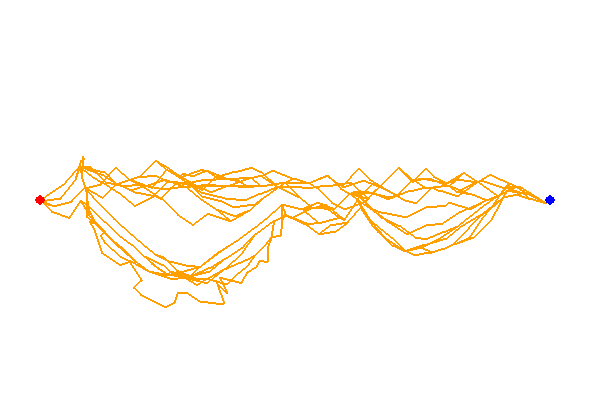
\includegraphics[width=\textwidth]{fig/sim8-nconvex/MORRTstar03-ALL.png}
		\caption{Pareto paths: weighted sum}
		\label{fig:sim:nonconvex:sols:a}
	\end{subfigure}  \\
	\begin{subfigure}[b]{0.45\linewidth}
		\centering
		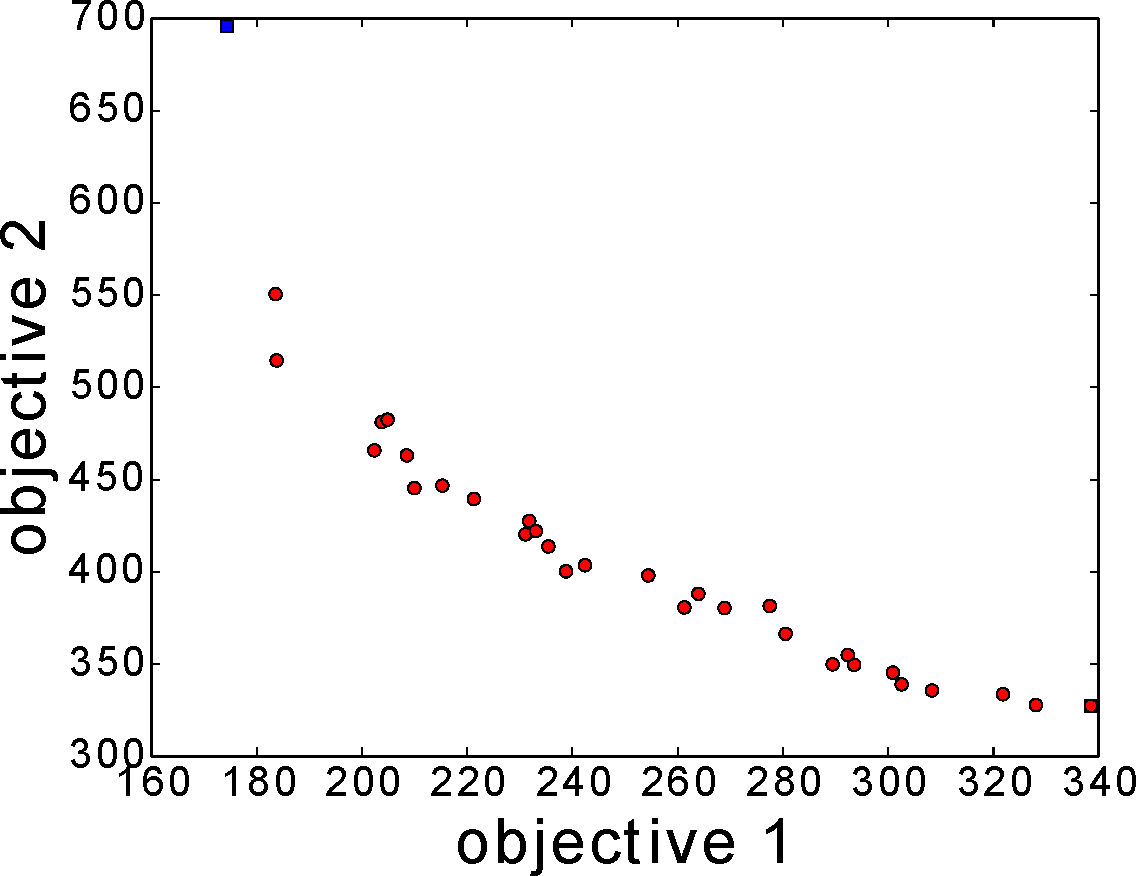
\includegraphics[width=\textwidth]{fig/sim9-nconvex/PF03-MORRT2.pdf}
		\caption{Pareto set: Tchebycheff}
		\label{fig:sim:nonconvex:pf:b}
	\end{subfigure} 
	\begin{subfigure}[b]{0.45\linewidth}
		\centering
		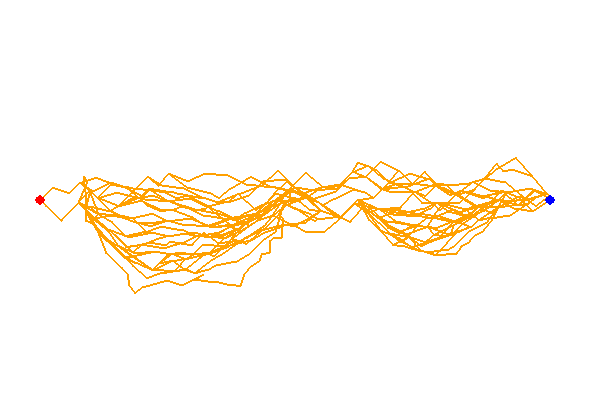
\includegraphics[width=\textwidth]{fig/sim9-nconvex/MORRTstar03-ALL.png}
		\caption{Pareto paths: Tchebycheff}
		\label{fig:sim:nonconvex:sols:b}
	\end{subfigure}
	\caption{Path planning with two conflicting objectives.}
	\label{fig:sim:nonconvex}
\end{figure}
\end{comment}

Finally, we evaluated how MORRF$^{*}$ performs three objectives: 
Euclidean distance and the two other objectives are shown in Figures~\ref{fig:sim:many:distance}-\ref{fig:sim:many:fitness2}.
As shown in Figure \ref{fig:sim:many}, the Pareto front uses the Utopia reference vector (Green point) to better approximate the Pareto set than the weighted sum approach, albeit in a somewhat noisy way.

\begin{figure}[h!]
	\centering
	\begin{subfigure}[b]{0.26\linewidth}
		\centering
		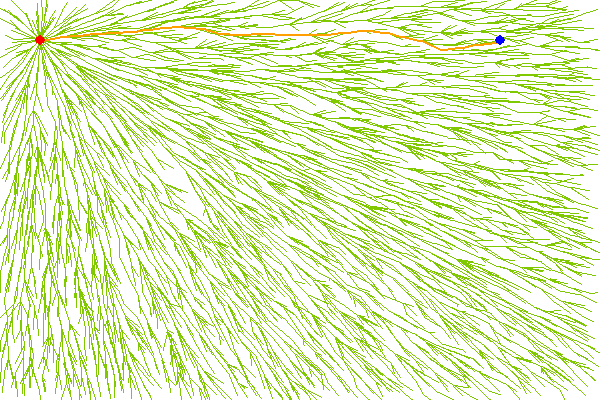
\includegraphics[width=\textwidth]{fig/sim6-3obj/MORRTstar02-0.png}
		\caption{Distance}
		\label{fig:sim:many:distance}
	\end{subfigure}
	\begin{subfigure}[b]{0.26\linewidth}
		\centering
		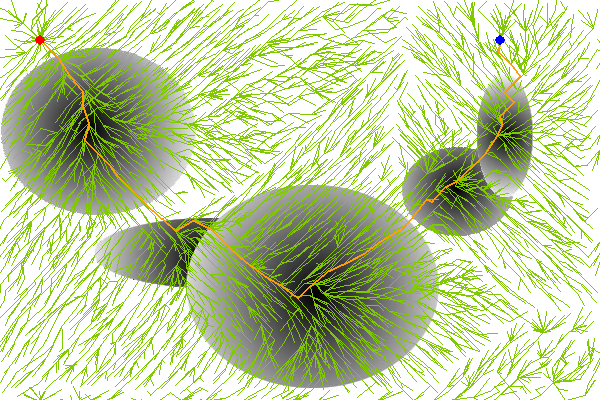
\includegraphics[width=\textwidth]{fig/sim6-3obj/MORRTstar02-1.png}
		\caption{Cost 1}
		\label{fig:sim:many:fitness1}
	\end{subfigure}
	\begin{subfigure}[b]{0.26\linewidth}
		\centering
		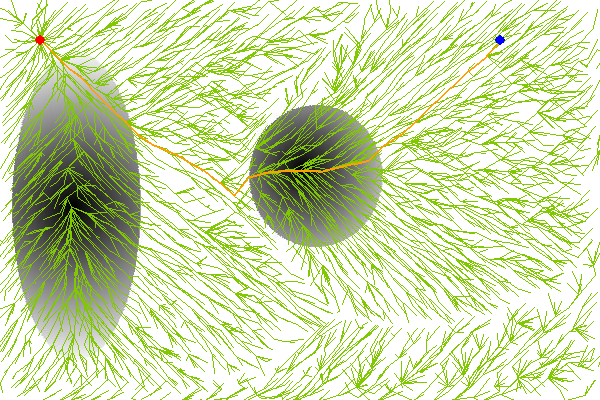
\includegraphics[width=\textwidth]{fig/sim6-3obj/MORRTstar02-2.png}
		\caption{Cost 2}
		\label{fig:sim:many:fitness2}
	\end{subfigure}  \\
	\begin{subfigure}[b]{0.35\linewidth}
		\centering
		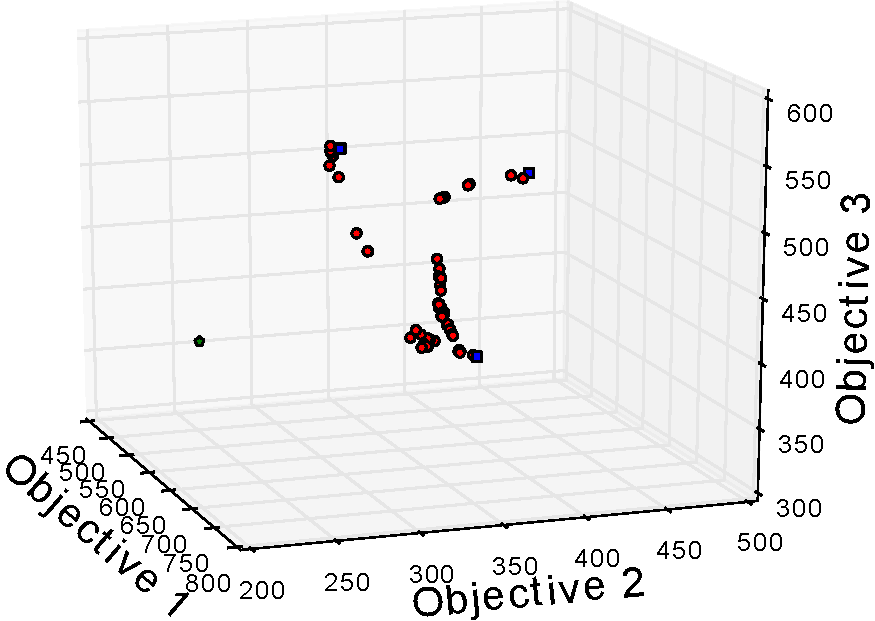
\includegraphics[width=\textwidth]{fig/sim6-3obj/PF06-MORRT.pdf}
		\caption{Pareto set: weighted sum}
		\label{fig:sim:many:pf:a}
	\end{subfigure}
	\begin{subfigure}[b]{0.35\linewidth}
		\centering
		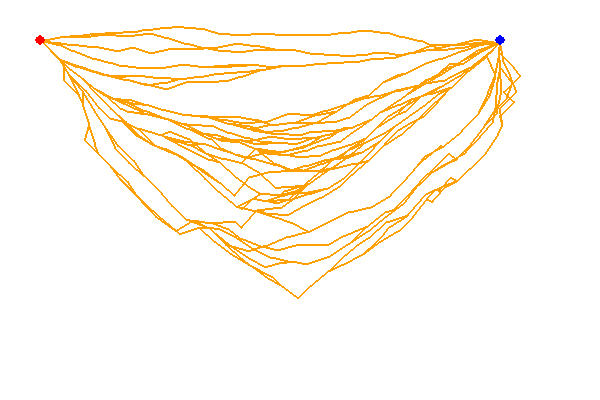
\includegraphics[width=\textwidth]{fig/sim6-3obj/MORRTstar02-ALL.png}
		\caption{Pareto paths: weighted sum}
		\label{fig:sim:many:sols:a}
	\end{subfigure}  \\
	\begin{subfigure}[b]{0.35\linewidth}
		\centering
		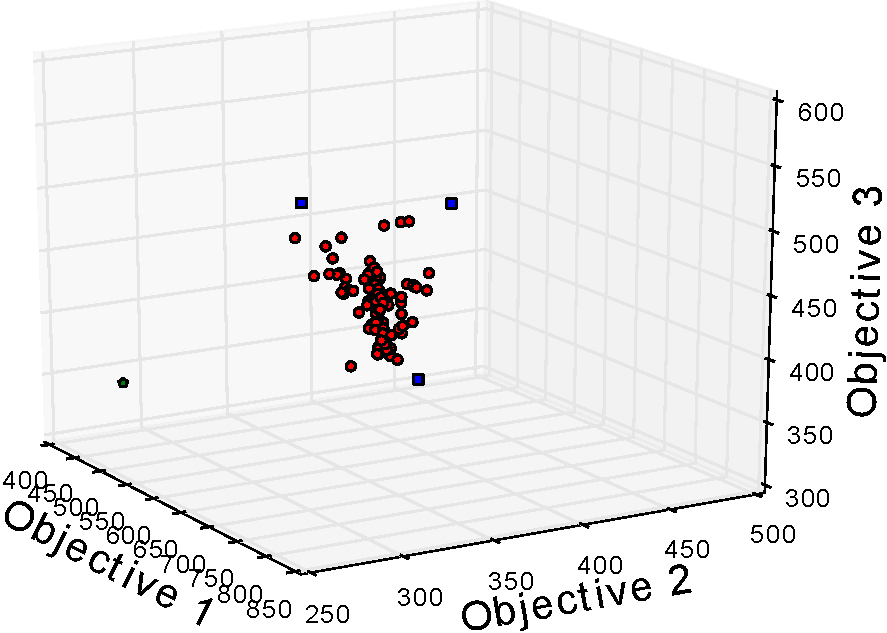
\includegraphics[width=\textwidth]{fig/sim7-3obj/PF07-MORRT2.pdf}
		\caption{Pareto set: Tchebycheff}
		\label{fig:sim:many:pf:b}
	\end{subfigure} 
	\begin{subfigure}[b]{0.35\linewidth}
		\centering
		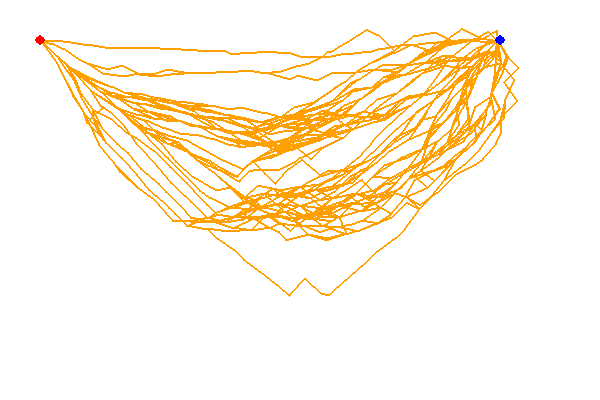
\includegraphics[width=\textwidth]{fig/sim7-3obj/MORRTstar02-ALL.png}
		\caption{Pareto paths: Tchebycheff}
		\label{fig:sim:many:sols:b}
	\end{subfigure}
	\caption{Path planning with three objectives.}
	\label{fig:sim:many}
\end{figure}

\section{Conclusion} 
\label{sec:conclusion}

This paper presented the MORRF$^{*}$ algorithm for the multi-objective path-planning problems on continuous spaces.
The algorithm blends principles from the RRT$^{*}$ algorithm with principles from multi-objective optimization to produce an algorithm that provides a reasonable approximation of the Pareto set, outperforms a common multi-objective optimization problem on a path-planning problem, and has guaranteed best-case performance.

Future work should extend the algorithm to include not only the weighted sum and Tchebycheff approach but also the the boundary intersection approach, which results from~\cite{4358754} suggest should have even better diversity.
MORRF$^{*}$ could also be made more efficient by, for example, using prior information to improve the set of sample points.
For example, when an objective includes minimizing Euclidean distance in the presence of obstacles, visibility graph techniques could be used to produce a prior set of sample points guaranteed to include the shortest path.
Additionally, if there is structure in the cost functions, which may be common in path-planning problems, then the sampling of new points could be based on information collected from the environment, allowing more search effort to be put in the more interesting regions.

Another area of future work is to combine MORRF$^{*}$ with Bellman's principle of optimality.
This could be done by setting a goal position as the root node in the algorithm and then generating a set of Pareto optimal paths.
The algorithm should then converge to the set of Pareto optimal from any vertex in the tree to the goal.
Additionally, if movement deviates from the original path, it should be very efficient to generate a new set of Pareto optimal paths from the new position to the goal position.

%\section*{Acknowledgments}
%Omitted for anonymous review.

\bibliographystyle{named}
\bibliography{reference}

\section{Appendix}

\subsection{Proof of Lemma \ref{lem:sub_tree:conv}}

\begin{proof}

\begin{figure}
\centering
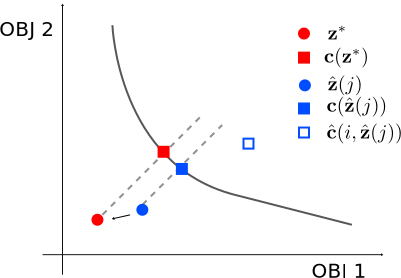
\includegraphics[width=0.4\linewidth]{fig/conv}
\caption{The convergence process of .}
\label{fig:conv}
\end{figure}

By Lemma \ref{lem:ref_tree:conv}, we have 
\begin{equation}
\lim_{j \to \infty} \lVert \bm{z}^{*} - \hat{\bm{z}} (j) \rVert = 0.
\end{equation}
By Lemma \ref{lem:sub_tree:conv}, we have
\begin{equation}
\lim_{i \to \infty} \hat{\bm{c}}( i, \hat{\bm{z}}(j) ) = \bm{c}( \hat{\bm{z}}(j) ).
\end{equation}


We have $ \bm{c}( \bm{z} ) $ 
is Lipschitz continuous.
\begin{equation}
\begin{aligned}
& \lim_{i \to \infty} \lVert \bm{c}( \bm{z}^{*} ) -  \hat{\bm{c}}( i, \hat{\bm{z}}(j) ) \rVert \\
= & \lVert \lim_{i \to \infty} \bm{c}( \bm{z}^{*} ) - \lim_{i \to \infty} \hat{\bm{c}}( i, \hat{\bm{z}}(j) ) \rVert \\
= & \lVert \bm{c}( \bm{z}^{*} ) - \bm{c}( \hat{\bm{z}}(j) ) \rVert \leq K \lVert \bm{z}^{*} - \hat{\bm{z}}(j) \rVert
\end{aligned}
\end{equation}
As $ j \to \infty $, we have $ \hat{\bm{z}}(j) \to \bm{z}^{*} $, thus $ \lim_{i \to \infty} \lVert \bm{c}( \bm{z}^{*} ) -  \hat{\bm{c}}( i, \hat{\bm{z}}(j) ) \rVert \to 0 $.
It means that 
\begin{equation}
P( \{ \lim_{ \substack{ i \to \infty \\ j \to \infty } } \bm{c}^{\rm SUB}_{m} (i , \hat{\bm{z}} (j) ) =  \bm{c}_{m}^{*}  \} ) = 1 .
\end{equation}
\end{proof}


\end{document}